\documentclass[aspectratio=169]{beamer}
\usetheme{AnnArbor}

\definecolor{degatered}{rgb}{0.902,0.22,0.161}
\setbeamercolor{titlelike}{parent=structure,fg=white,bg=degatered}
\setbeamercolor*{palette primary}{bg=degatered!50!black,fg=white}
\setbeamercolor*{palette secondary}{bg=degatered!40!black,fg=white}
\setbeamercolor*{palette tertiary}{bg=degatered!30!black,fg=white}
\setbeamercolor*{palette quaternary}{bg=degatered!20!black,fg=white}
\setbeamercolor{frametitle}{bg=degatered}
\setbeamercolor{frametitle right}{bg=degatered!60!black}
\setbeamertemplate{bibliography item}{\insertbiblabel}

\usepackage{tikz}

\title{\textbf{\underline{Degate}}}
\subtitle{The stakes and challenges of silicon reverse engineering \\ \url{https://www.degate.org}}
\titlegraphic{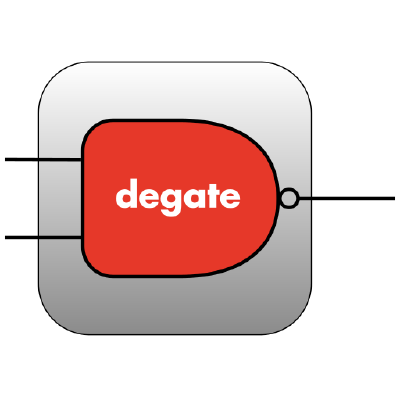
\includegraphics[width=2cm]{res/degate.png}}
\author{\textbf{D.~Bachelot}}
\date{\textbf{\underline{Degate Community}},\\ 2024}
\logo{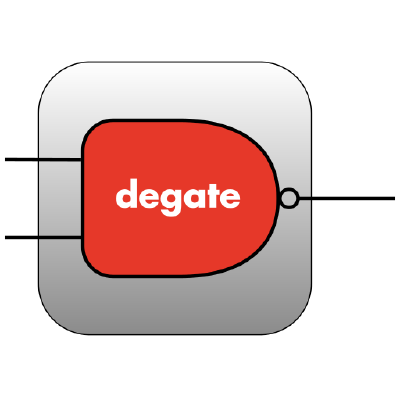
\includegraphics[scale=0.08]{res/degate.png}}

\AtBeginSection[ ]
{
	\begin{frame}{}
		\tableofcontents[currentsection]
	\end{frame}
}

\begin{document}
	
%%%%%%%%%%%%%%%%%%%%%%%%%%%%%%%%%%%%%%%%%%%%%%%%%%%%%%%%%%%%%%%%%%%%%%%%%%%%%%%%
%%%%%%%%%%%%%%%%%%%%%%%%%%%%%%%%%%%%%%%%%%%%%%%%%%%%%%%%%%%%%%%%%%%%%%%%%%%%%%%%
%%%%%%%%%%%%%%%%%%%%%%%%%%%%%%%%%%%%%%%%%%%%%%%%%%%%%%%%%%%%%%%%%%%%%%%%%%%%%%%%

%%%%%%%%%%%%%%%%%%%%%%%%%%%%%%%%%%%%%%%%%%%%%%%%%%
\begin{frame}[plain]
    \maketitle
\end{frame}
%%%%%%%%%%%%%%%%%%%%%%%%%%%%%%%%%%%%%%%%%%%%%%%%%%

%%%%%%%%%%%%%%%%%%%%%%%%%%%%%%%%%%%%%%%%%%%%%%%%%%%%%%%%%%%%%%%%%%%%%%%%%%%%%%%%

\begin{frame}{}
	\tableofcontents
\end{frame}

%%%%%%%%%%%%%%%%%%%%%%%%%%%%%%%%%%%%%%%%%%%%%%%%%%%%%%%%%%%%%%%%%%%%%%%%%%%%%%%%
%%%%%%%%%%%%%%%%%%%%%%%%%%%%%%%%%%%%%%%%%%%%%%%%%%%%%%%%%%%%%%%%%%%%%%%%%%%%%%%%
%%%%%%%%%%%%%%%%%%%%%%%%%%%%%%%%%%%%%%%%%%%%%%%%%%%%%%%%%%%%%%%%%%%%%%%%%%%%%%%%

\section{Silicon Chips Reverse Engineering}

%%%%%%%%%%%%%%%%%%%%%%%%%%%%%%%%%%%%%%%%%%%%%%%%%%%%%%%%%%%%%%%%%%%%%%%%%%%%%%%%

	\subsection{Introduction}
	
	%%%%%%%%%%%%%%%%%%%%%%%%%%%%%%%%%%%%%%%%%%%%%%%%%%
	
	\begin{frame}{}
		\tableofcontents[currentsection, currentsubsection]
	\end{frame}
	
	%%%%%%%%%%%%%%%%%%%%%%%%%%%%%%%%%%%%%%%%%%%%%%%%%%
	\begin{frame}{What is Silicon Chips RE?}
		\begin{tabular}{cl}  
			
			\begin{tabular}{c}
				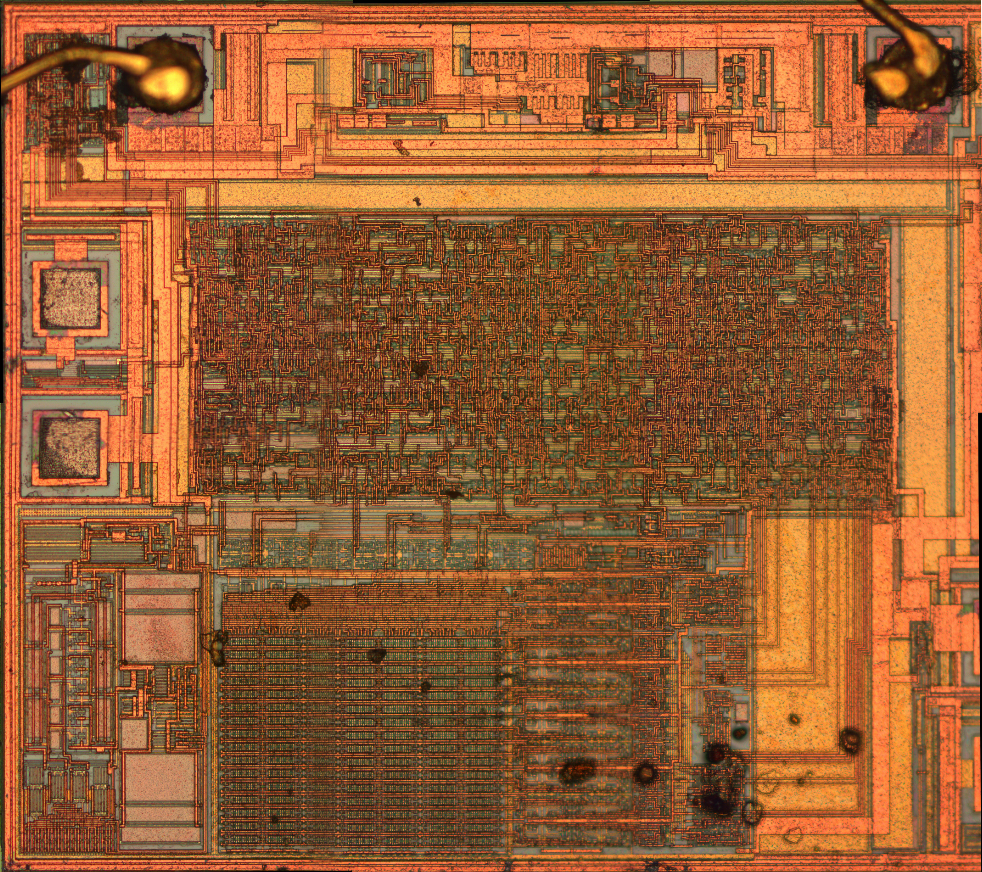
\includegraphics[width=5.2cm]{res/chip_example.png}
			\end{tabular}
			
			& \begin{tabular}{l}
				\parbox{0.5\linewidth}{\scriptsize
					Same idea than with software RE (from binary, to assembly and to code), silicon chip RE go \textbf{from silicon}, \textbf{to images}, \textbf{to transistors}, \textbf{to gates}, \textbf{to netlist} and \textbf{to algorithm}. \\
		
					With proper preparation and knowledge, we can go into silicon, \textbf{analyze transistors}, \textbf{retrieve gates/wires/vias} and \textbf{reconstruct implemented algorithms}. This can be used to \textbf{analyze old hardware}, build \textbf{software emulators}, search for \textbf{vulnerabilities} and \textbf{backdoors}, \textbf{break/test a protection}, \textbf{secret extraction} or \textbf{check intellectual property}. \\
					
					\textbf{Used in IC industry} for \textbf{fault/failure detection} \& analysis, but \textbf{not at the same scale}.
				}
			\end{tabular}
		
		\end{tabular}
		
		\begin{figure}[!ht]
			\centering
			\resizebox{0.7\textwidth}{!}{%
				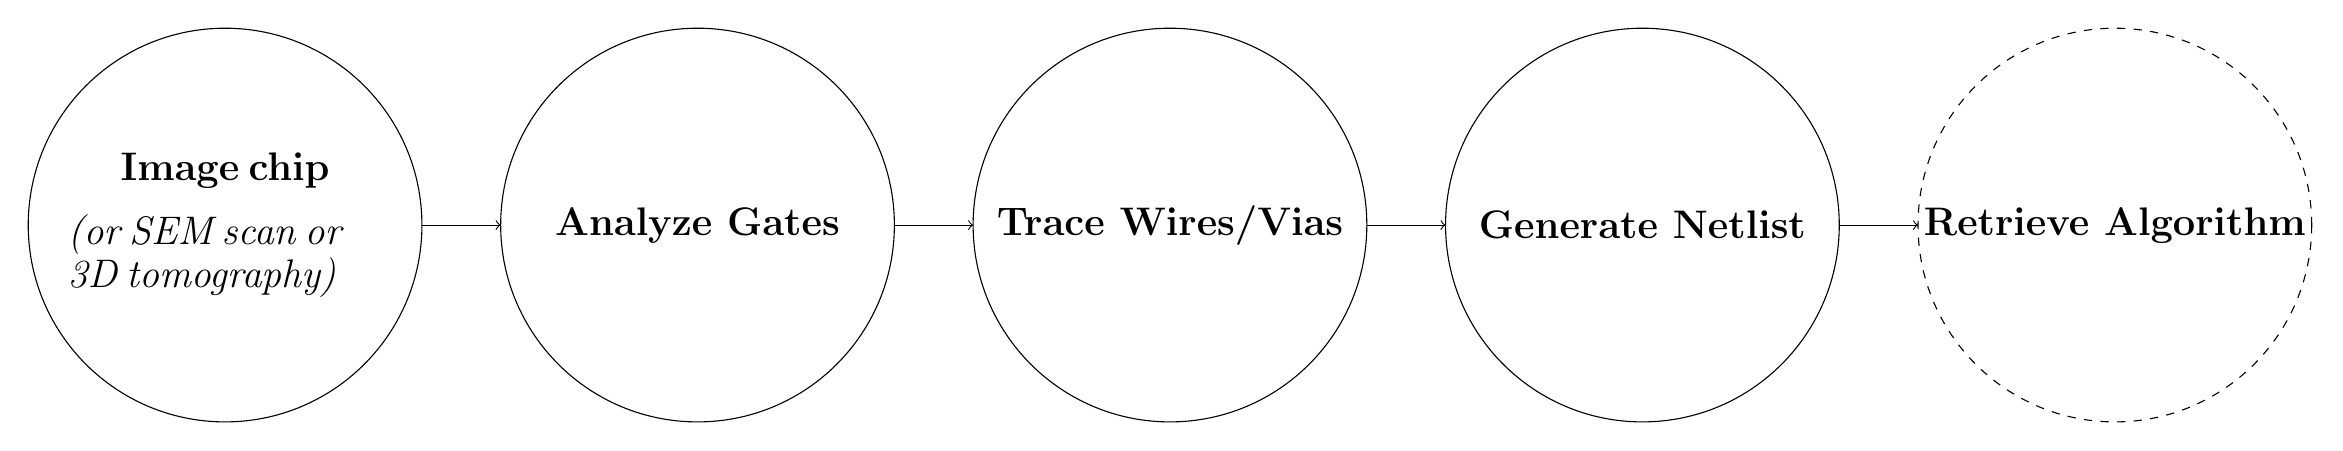
\begin{tikzpicture}
					\tikzstyle{every node}=[font=\normalsize]
					\draw  (10.5,17.75) circle (2.5cm) node [text width=4cm]
					{ \Large
						\centering \textbf{Image chip} \\
						\vspace{3mm}
						\textit{(or SEM scan or 3D tomography)}
					} ;
					\draw  (16.5,17.75) circle (2.5cm) node {\Large \textbf{Analyze Gates}} ;
					\draw  (22.5,17.75) circle (2.5cm) node {\Large \textbf{Trace Wires/Vias}} ;
					\draw  (28.5,17.75) circle (2.5cm) node {\Large \textbf{Generate Netlist}} ;
					\draw [, dashed] (34.5,17.75) circle (2.5cm) node {\Large \textbf{Retrieve Algorithm}} ;
					\draw [->] (13,17.75) -- (14,17.75);
					\draw [->] (19,17.75) -- (20,17.75);
					\draw [->] (25,17.75) -- (26,17.75);
					\draw [->] (31,17.75) -- (32,17.75);
				\end{tikzpicture}
			}%
		\end{figure}
	\end{frame}
	%%%%%%%%%%%%%%%%%%%%%%%%%%%%%%%%%%%%%%%%%%%%%%%%%%
	
	%%%%%%%%%%%%%%%%%%%%%%%%%%%%%%%%%%%%%%%%%%%%%%%%%%
	\begin{frame}{How to Access Silicon?}	
		Can be very costly (plasma \& laser) and destructive... But also accessible with simpler methods (like chemical/mechanical). More on \cite{SiliconPron}.
		
		\begin{enumerate}
			\item \textbf{Decapsulation} (heat, acid, mechanical, plasma, laser...)
			\item \textbf{Delayering} (chemical, abrasive, laser, plasma...)
			\item \textbf{Cleaning} (ultrasound, acid...)
		\end{enumerate}
		
		\begin{center}
			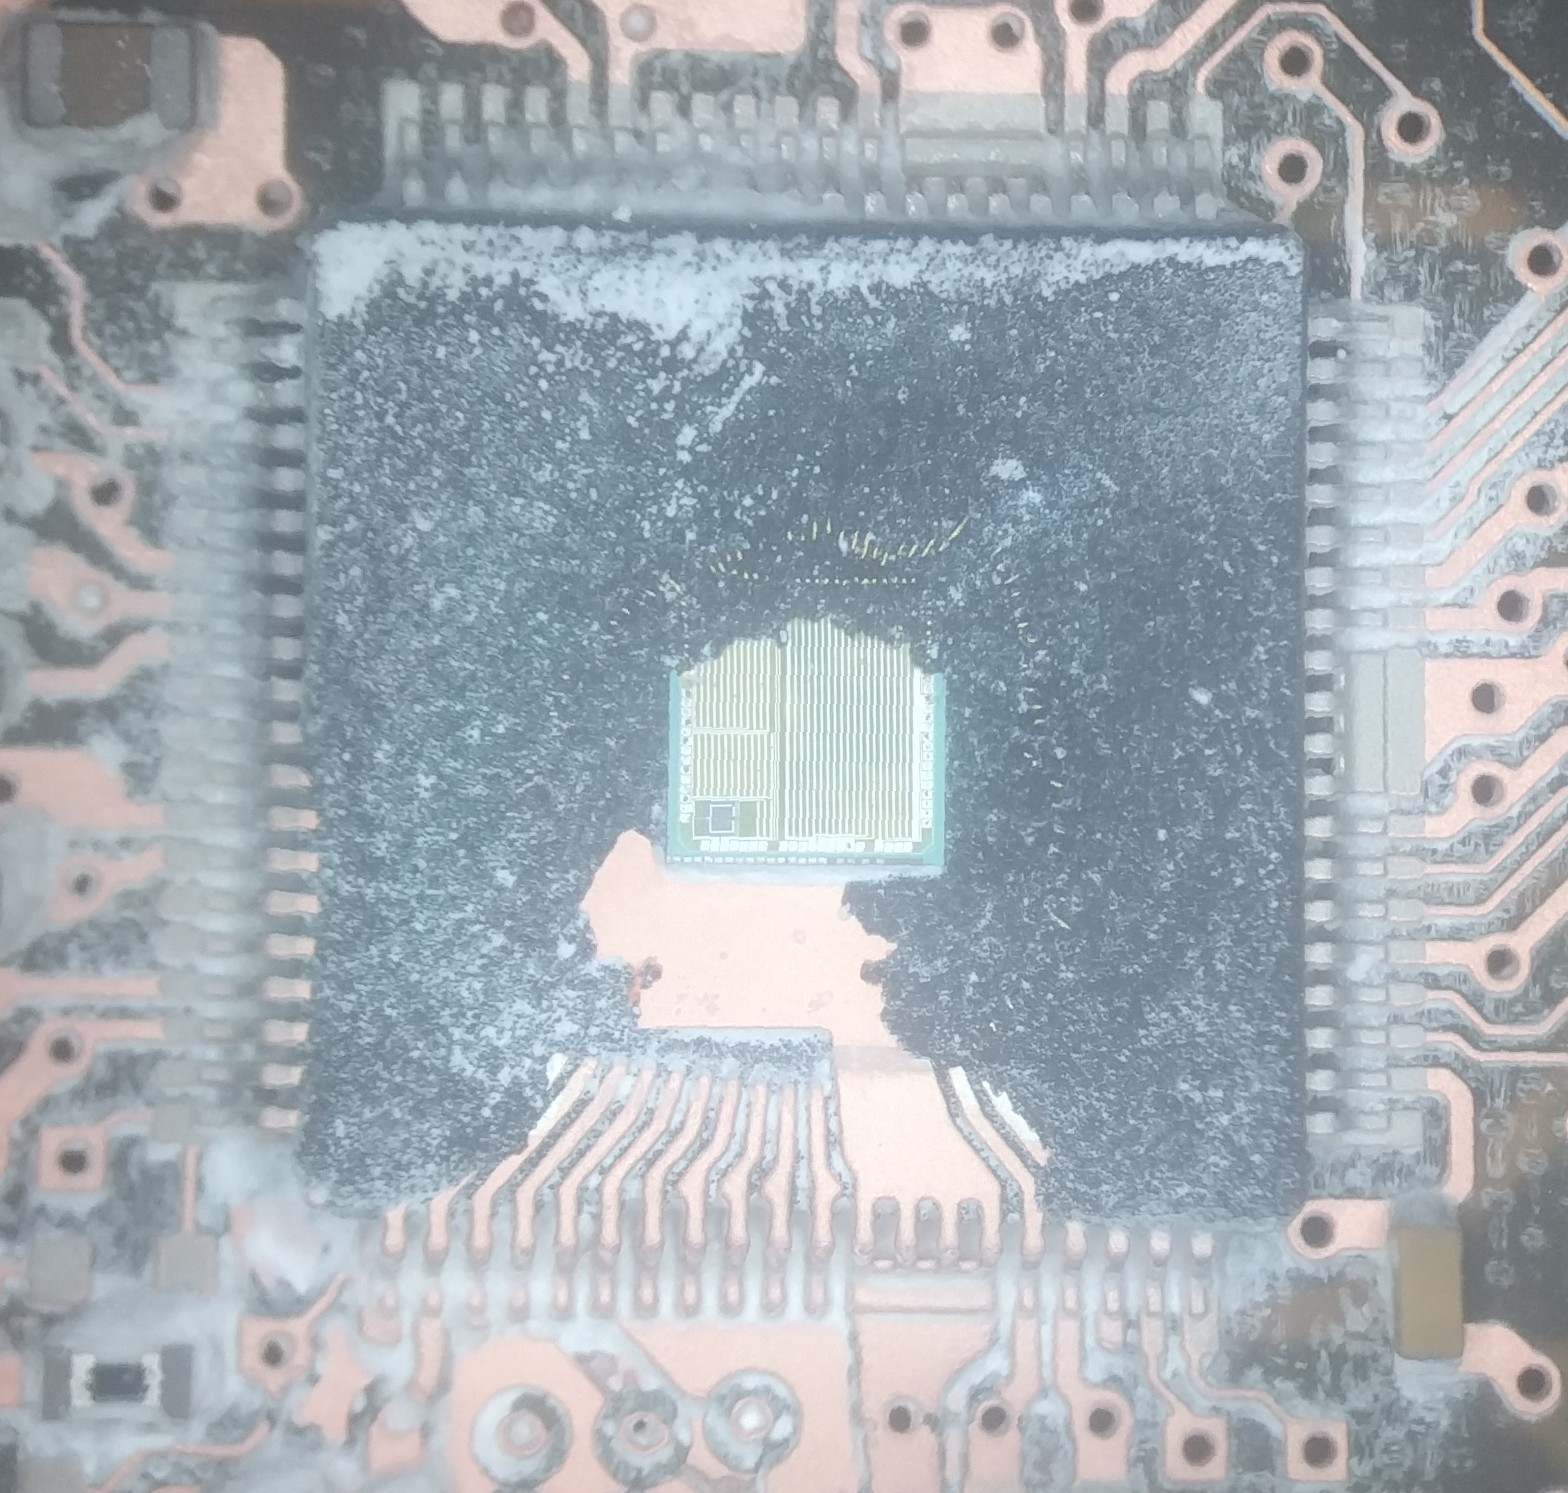
\includegraphics[width=4cm]{res/decap.jpg}
			\cite{Holler2017}
			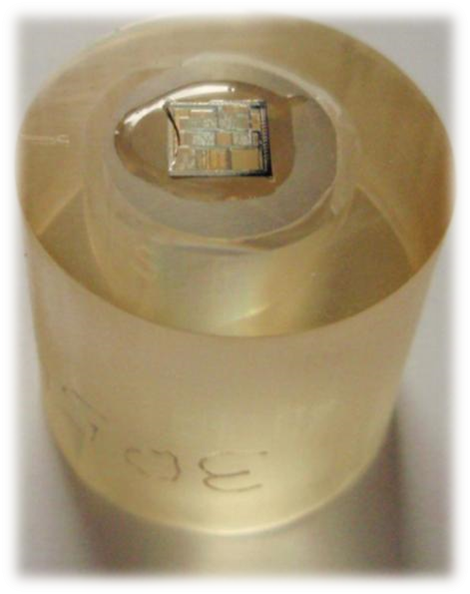
\includegraphics[width=3cm]{res/delayer.png}
			\cite{KarstenNohl2009}
			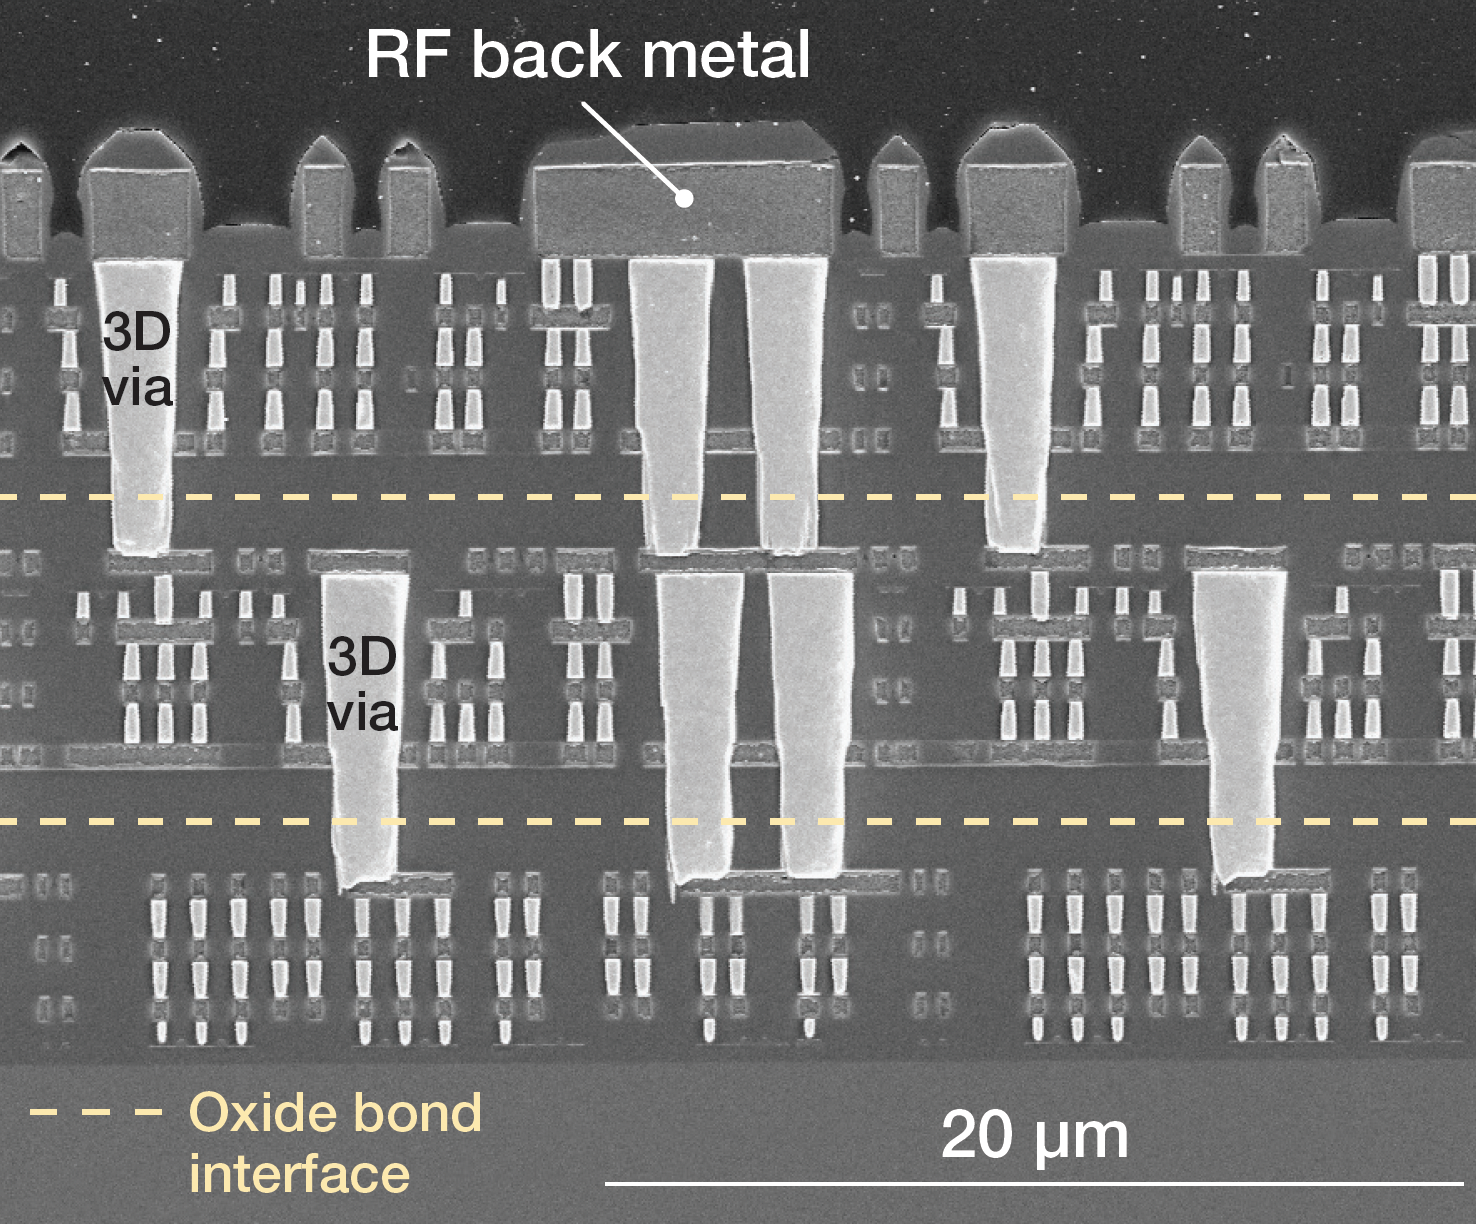
\includegraphics[width=4.5cm]{res/delayered.png}
			\tiny MIT
		\end{center}
	\end{frame}
	%%%%%%%%%%%%%%%%%%%%%%%%%%%%%%%%%%%%%%%%%%%%%%%%%%
	
	%%%%%%%%%%%%%%%%%%%%%%%%%%%%%%%%%%%%%%%%%%%%%%%%%%
	\begin{frame}{How to Retrieve Images?}
		Using each layer (invasive) or directly using the chip (non-invasive):
		\begin{itemize}
			\item Take very-high resolution images from \textbf{optical microscope} (basic, confocal) ;
			\item Scan from an \textbf{electron microscope} (SEM, TEM...) ;
			\item Generate a 3D model using \textbf{electron tomography} ;
		\end{itemize}
		
		\begin{center}
			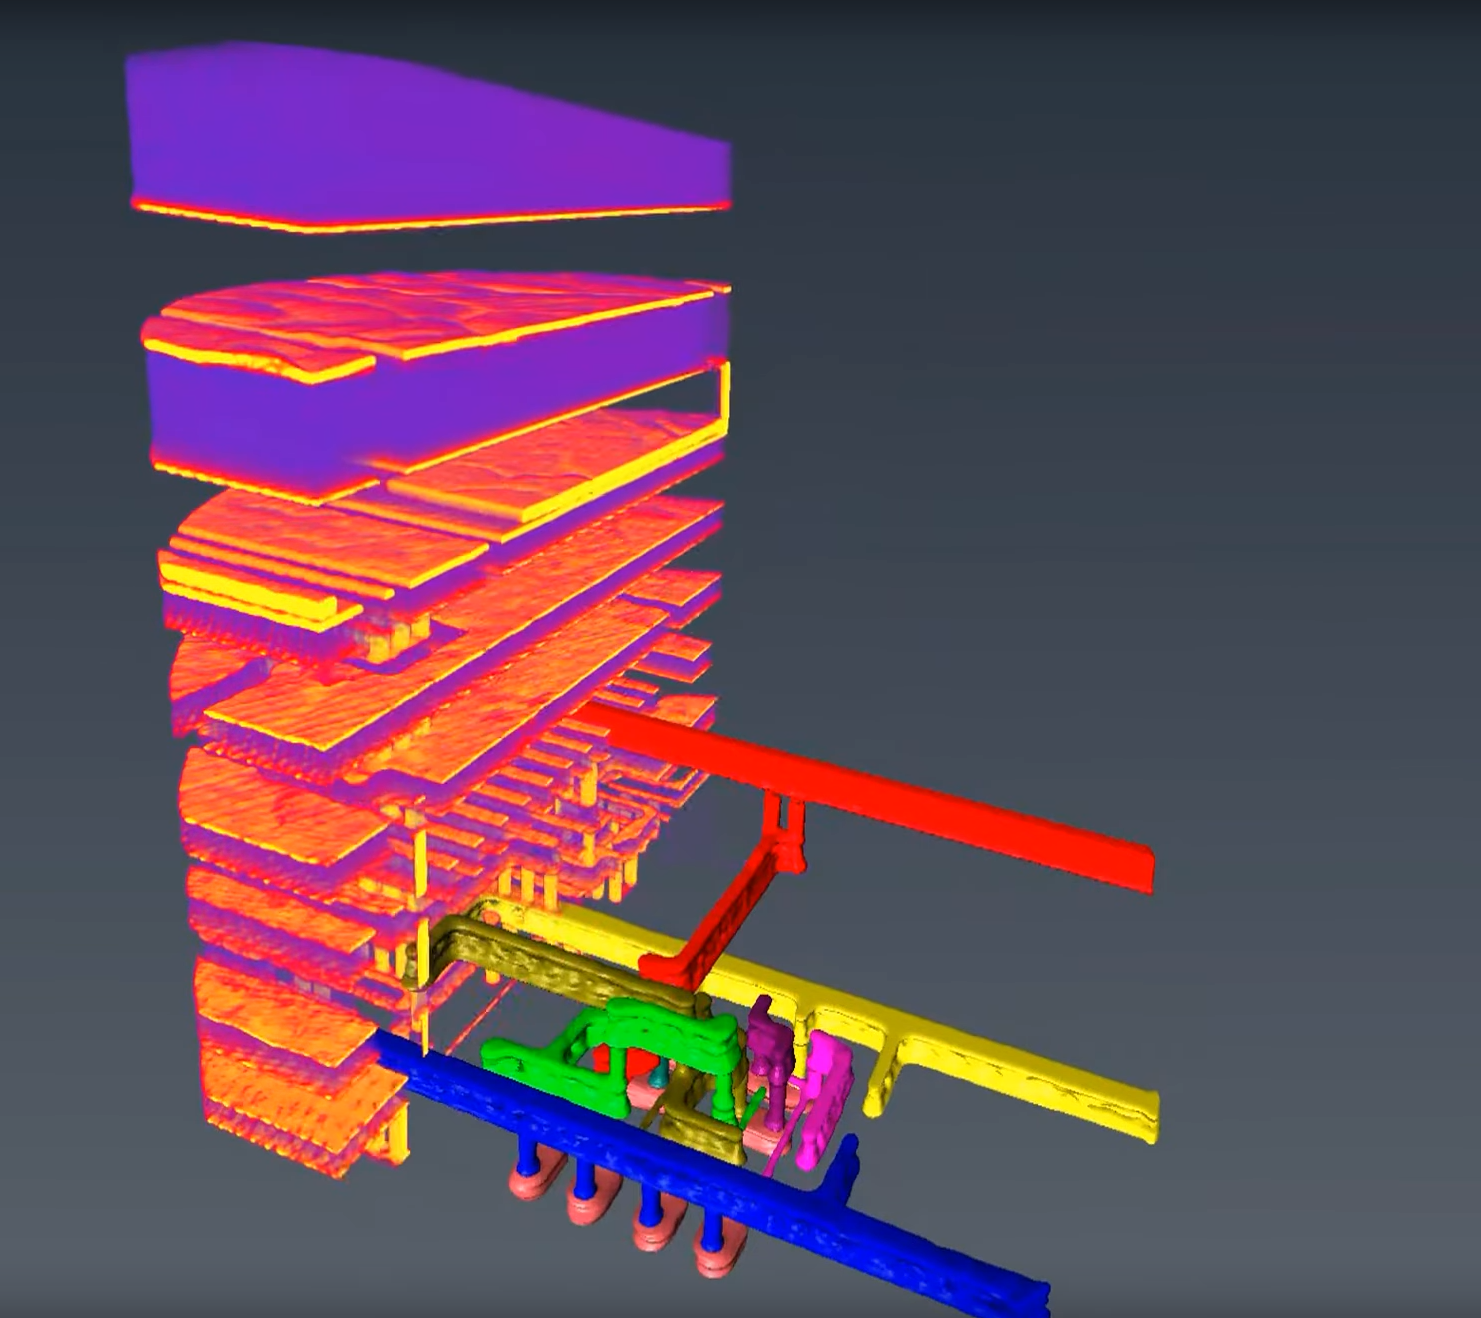
\includegraphics[width=5cm]{res/3d_1.png}
			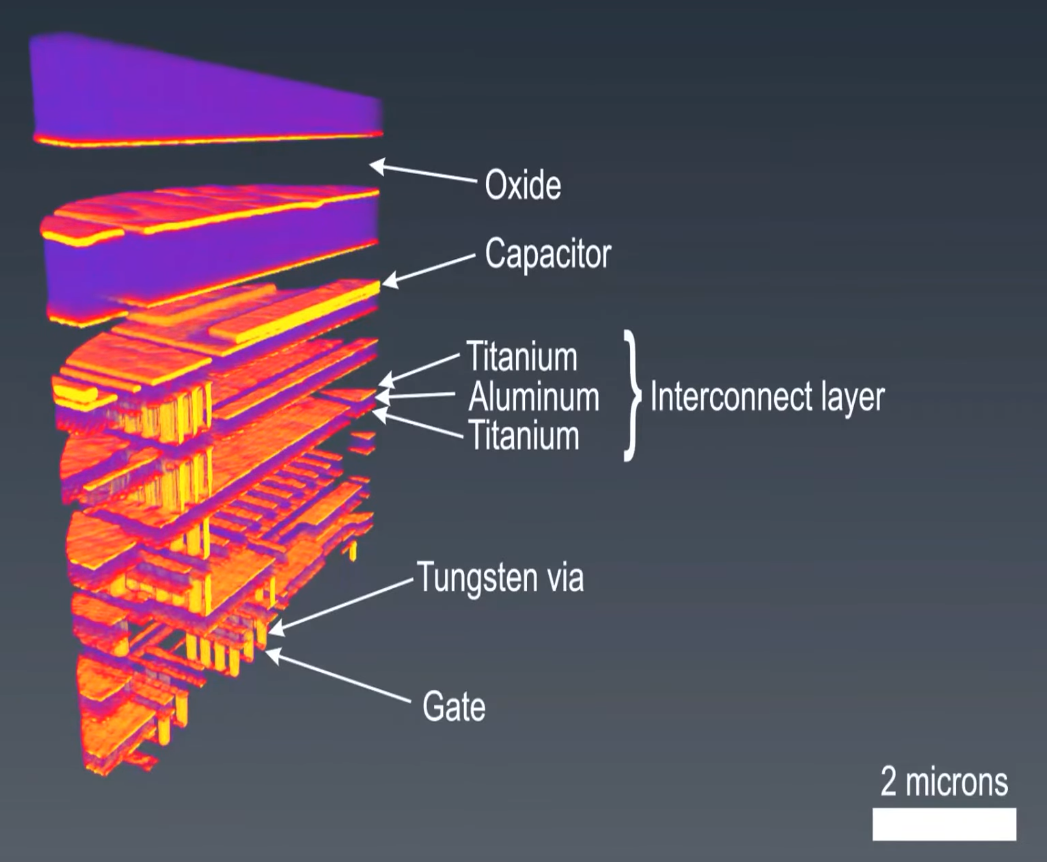
\includegraphics[width=5.4cm]{res/3d_2.png}
			\cite{Holler2017}
		\end{center}
	\end{frame}
	%%%%%%%%%%%%%%%%%%%%%%%%%%%%%%%%%%%%%%%%%%%%%%%%%%
	
	%%%%%%%%%%%%%%%%%%%%%%%%%%%%%%%%%%%%%%%%%%%%%%%%%%
	\begin{frame}{How to Perform the Analysis?}
		
		\begin{tabular}{cl}  
			
			\begin{tabular}{c}
				\parbox{0.5\linewidth}{
					\vspace{-3mm}
					Overview:
					\begin{enumerate}
						\item Choose a \textbf{zone of interest},
						\item Identify each \textbf{gate type}, annotate, and place in a \textbf{"gate library"},
						\item Find other \textbf{gates instance} from gate library,
						\item Link gates by tracing \textbf{wires and vias},
						\item Export to \textbf{netlist} (e.g. by translating each gate to VHDL/Verilog code).
					\end{enumerate}
				}
			\end{tabular}
			
			& \begin{tabular}{l}
				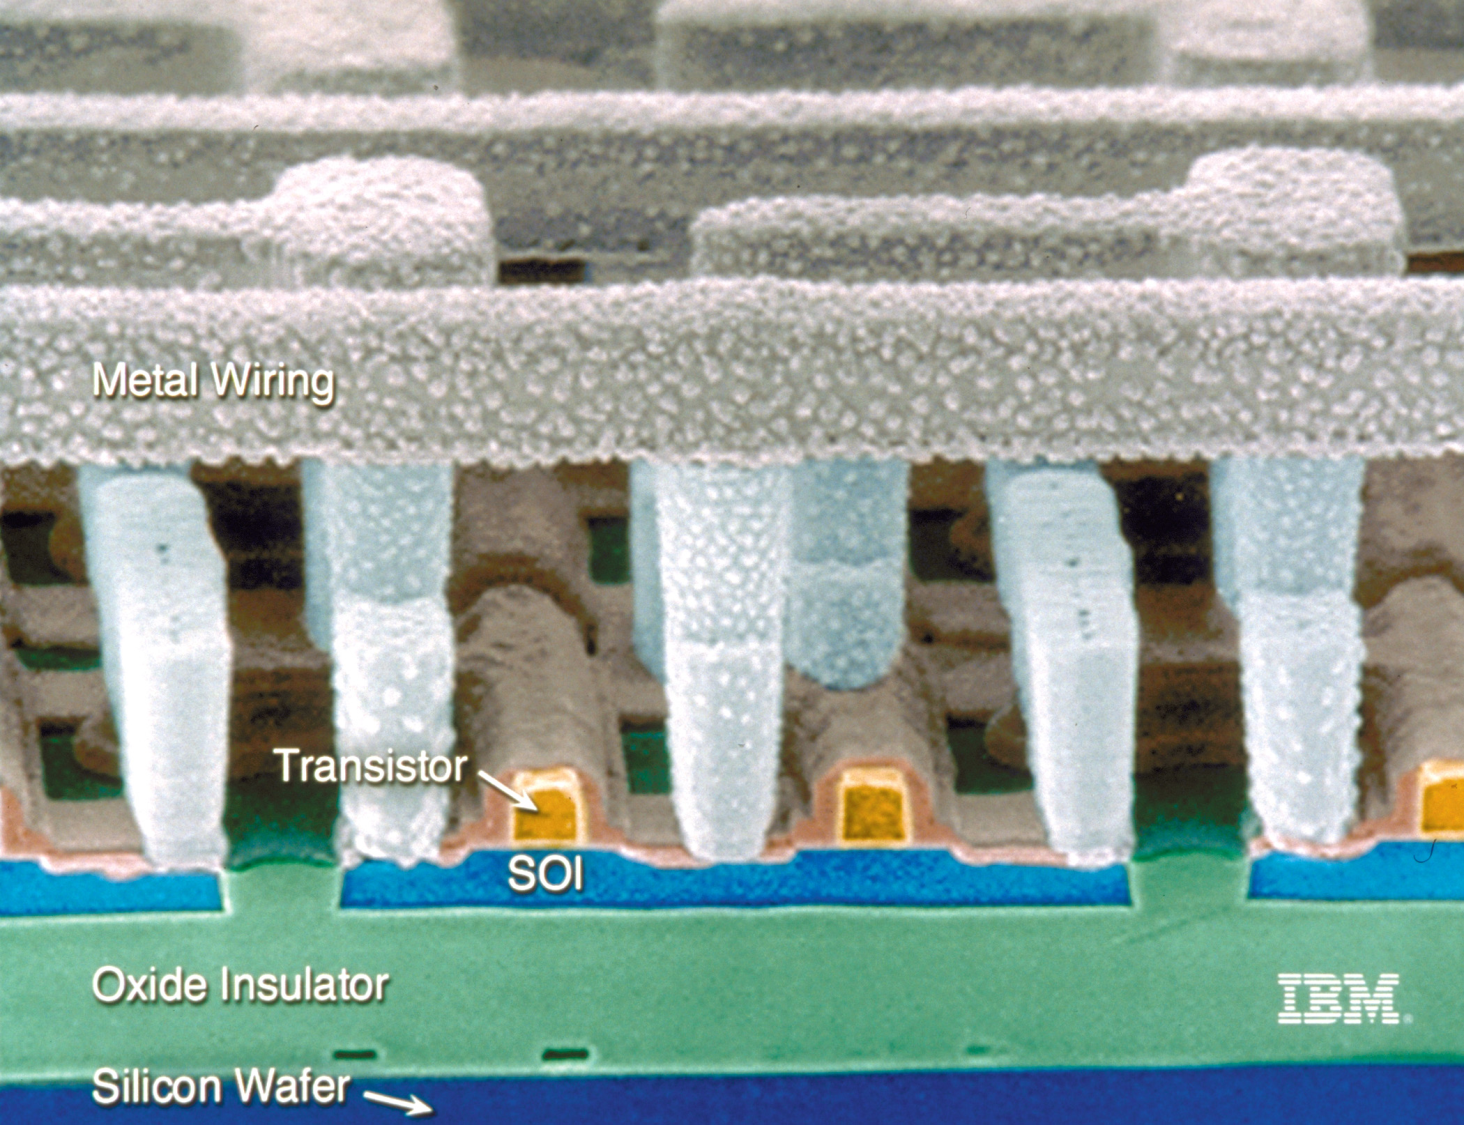
\includegraphics[width=6.25cm]{res/transistor.png}
			\end{tabular}
			
		\end{tabular}
	\end{frame}
	%%%%%%%%%%%%%%%%%%%%%%%%%%%%%%%%%%%%%%%%%%%%%%%%%%
	
	%%%%%%%%%%%%%%%%%%%%%%%%%%%%%%%%%%%%%%%%%%%%%%%%%%
	\begin{frame}{How to identify a transistor?}
		
		\begin{tabular}{cl}  
			
			\begin{tabular}{c}
				\parbox{0.5\linewidth}{\small
					\begin{enumerate}
						\item Search, at transistor layer, for \textbf{doped zones}.
						\item Spot the \textbf{zebras}.
						\item Use logic to identify the \textbf{type of each transistor} (e.g. PMOS are bigger to compensate with lower hole mobility).
						\item Search for \textbf{wires} (to identify inputs and outputs).
					\end{enumerate}
				}
			\end{tabular}
			
			& \begin{tabular}{l}
				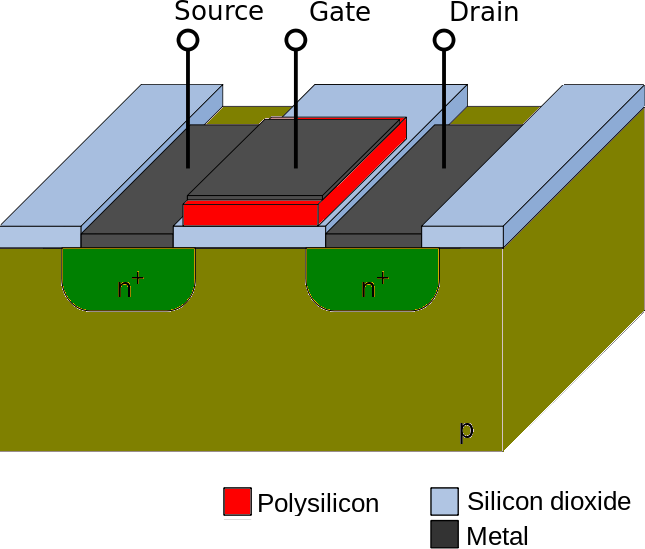
\includegraphics[width=4cm]{res/npn.png}
				\vspace{10mm} 
				\tiny (NMOS, \textit{Wikipedia})
			\end{tabular}
			
		\end{tabular}
		
		\centering
		\hspace{-40mm}
		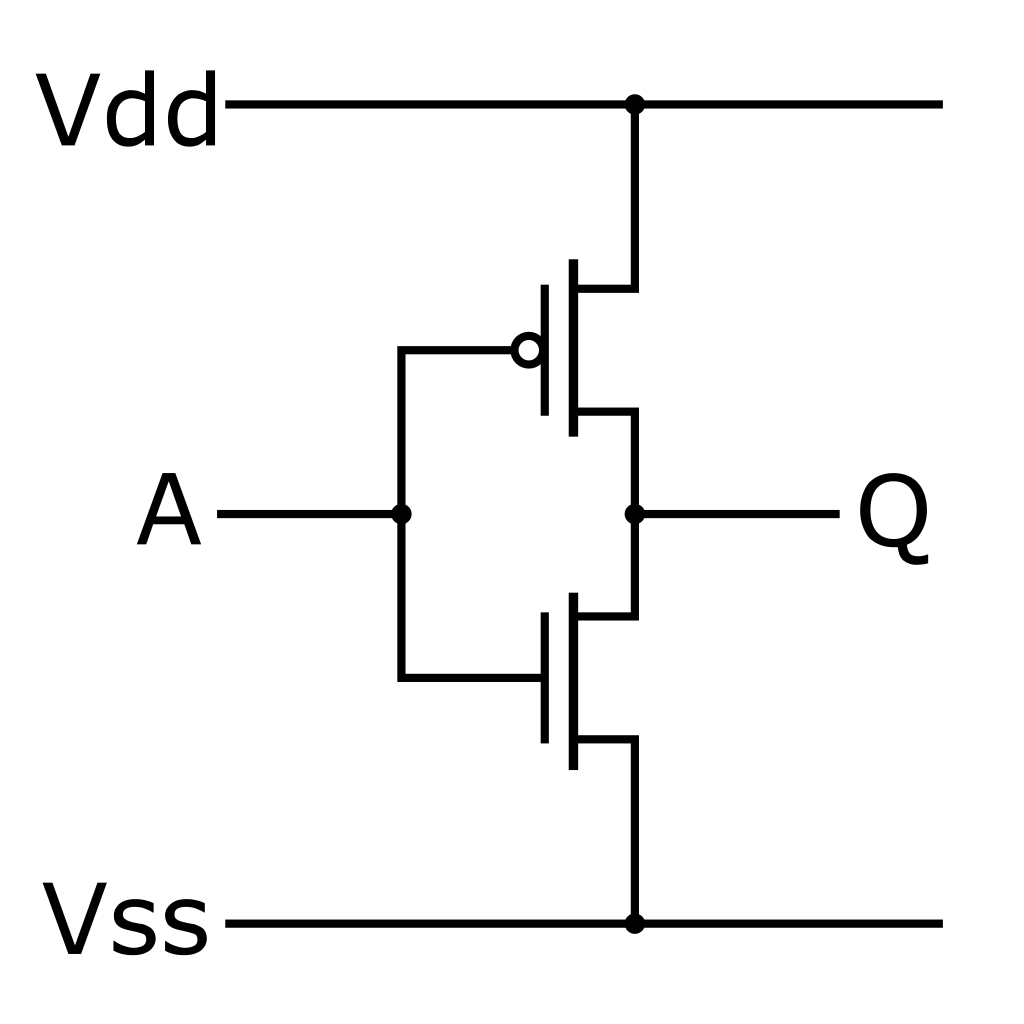
\includegraphics[width=2.5cm]{res/cmos.png}
		\tiny (Inverter, \textit{Wikipedia})
		\hspace{6mm}
		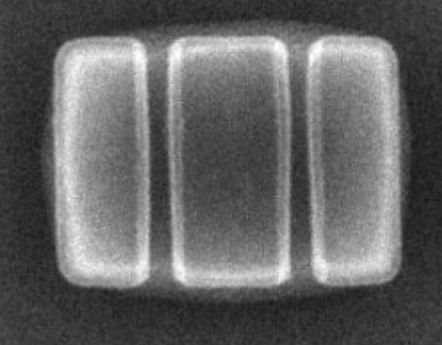
\includegraphics[width=3cm]{res/dopant_pmos.png}
		\tiny (PMOS \cite{YenerBulent2014})
	\end{frame}
	%%%%%%%%%%%%%%%%%%%%%%%%%%%%%%%%%%%%%%%%%%%%%%%%%%
	
	%%%%%%%%%%%%%%%%%%%%%%%%%%%%%%%%%%%%%%%%%%%%%%%%%%
	\begin{frame}{How to Identify a Gate?}
		
		\begin{tabular}{ccc}  
			\begin{tabular}{c}  
				
				\begin{tabular}{ccc}
					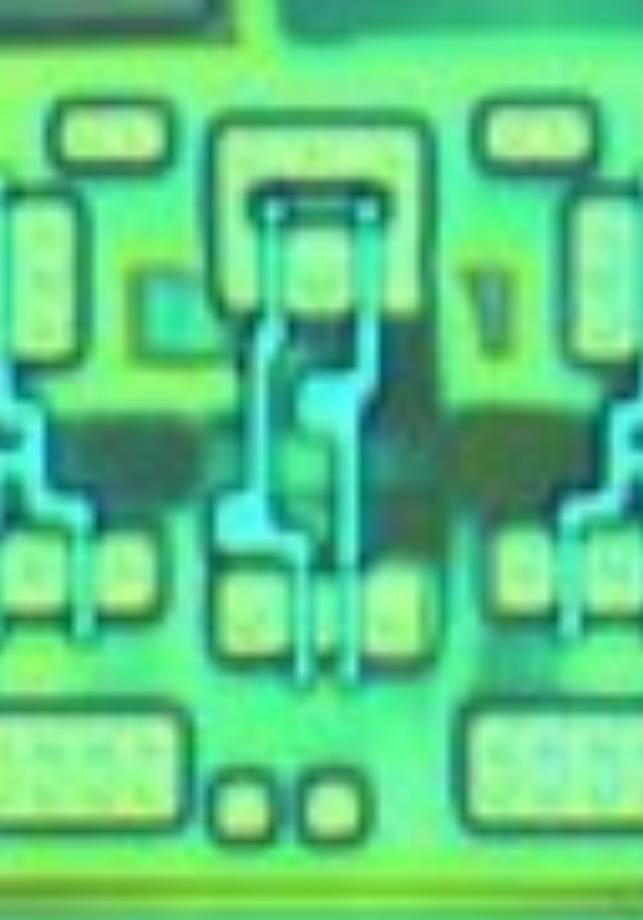
\includegraphics[width=1.75cm]{res/ana_1.png} &
					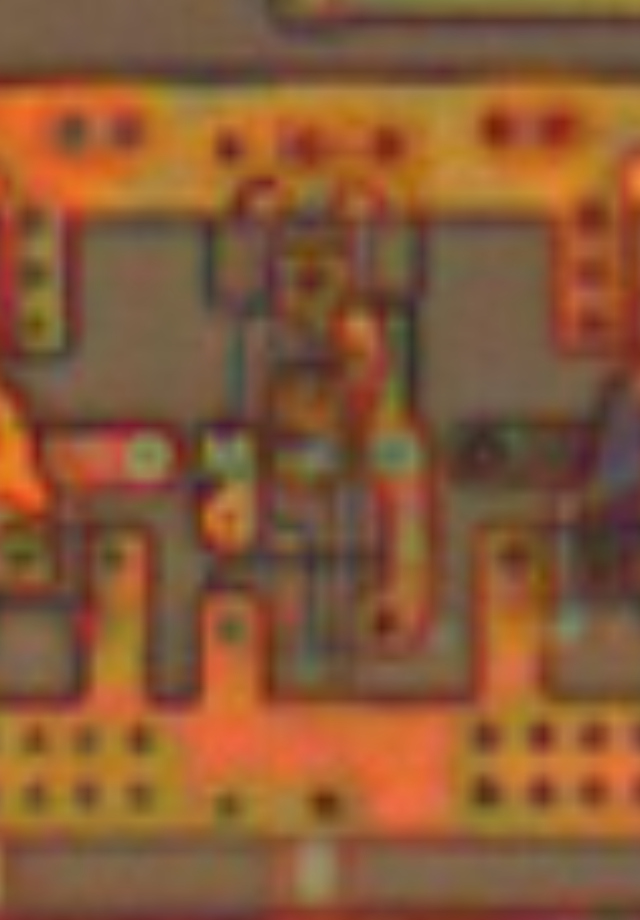
\includegraphics[width=1.75cm]{res/ana_2.png} &
					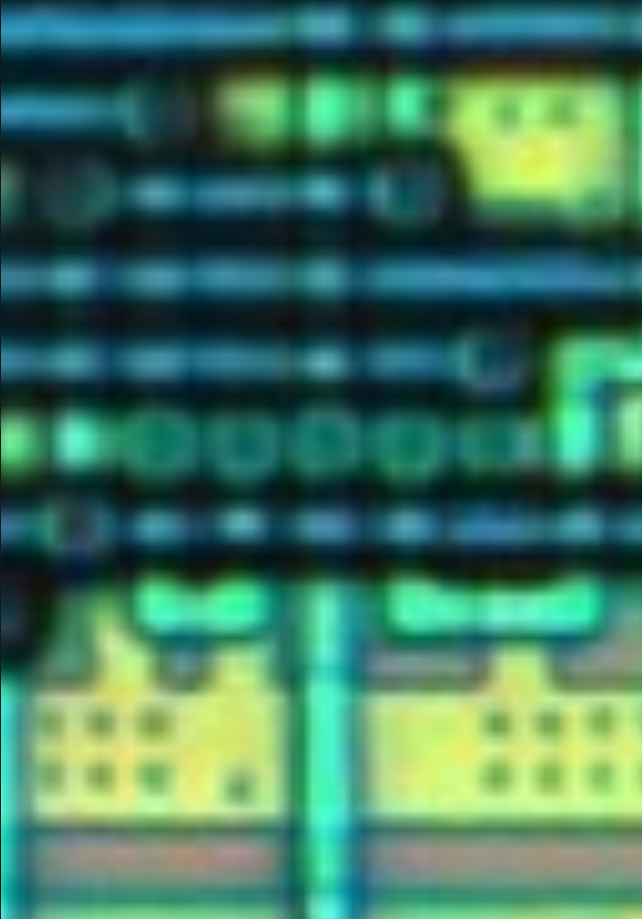
\includegraphics[width=1.75cm]{res/ana_3.png} \\
					\tiny Transistor layer &
					\tiny Logic layer &
					\tiny Metal layer \\
				\end{tabular} \\
				
				$\Downarrow$ \\
				
				\begin{tabular}{cc}
					\tiny
					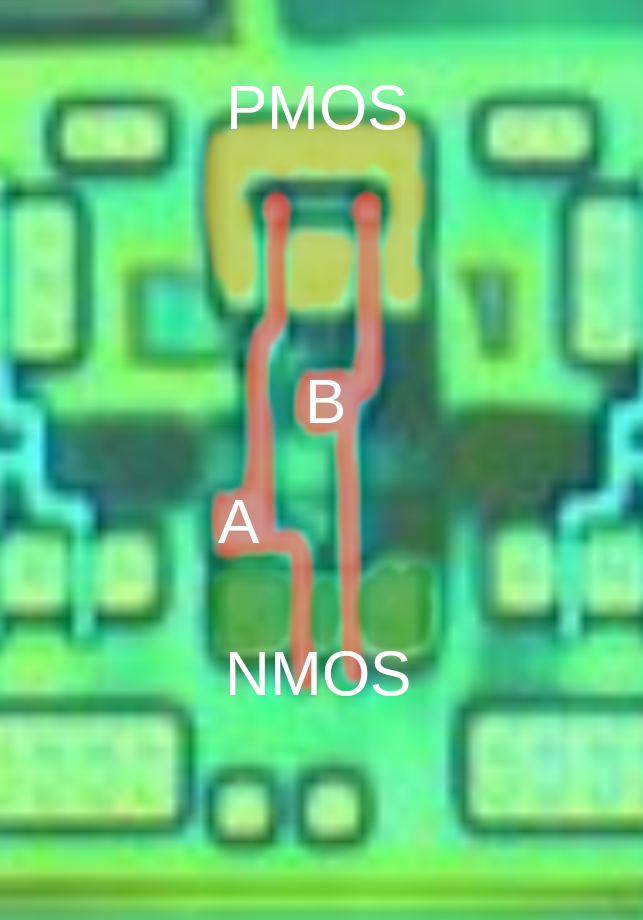
\includegraphics[width=1.75cm]{res/post_ana_1.png} &
					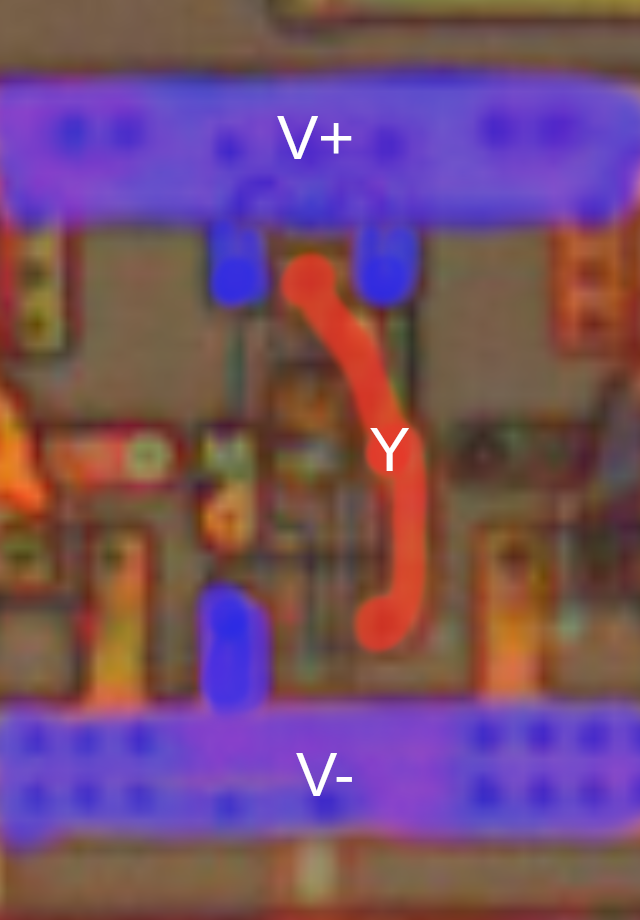
\includegraphics[width=1.75cm]{res/post_ana_2.png} \\
					\tiny P \& N zones and 2 inputs &
					\tiny V+ \& V-, and output \\
				\end{tabular}
				
			\end{tabular} &
			
			$\Rightarrow$
			
			& 
			
			\ensuremath{\vcenter{\hbox{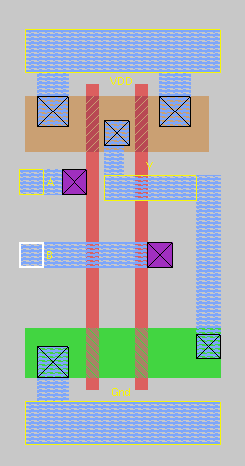
\includegraphics[width=3cm]{res/ana_layout.png}}}}
			{\tiny\cite{SiliconZoo}}
			$\Rightarrow$
			\begin{tabular}{c}
				\textbf{NAND gate!} \\
				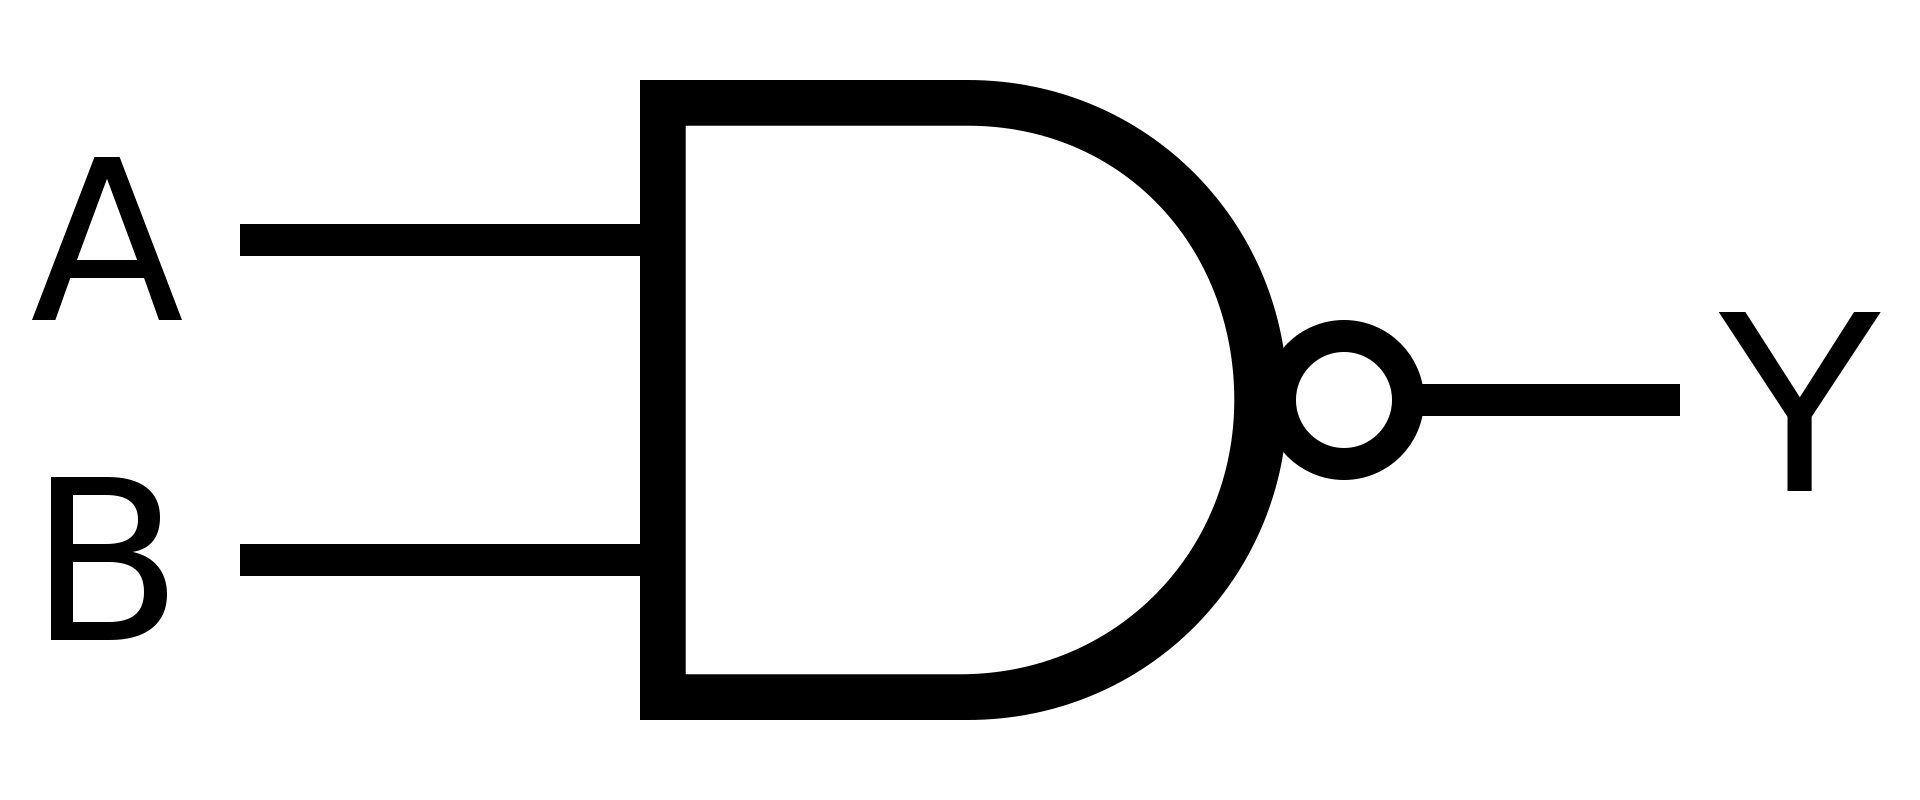
\includegraphics[width=2.5cm]{res/nand.png} \\
				\begin{tabular}{ | c | c || c | }
					\hline
					A & B & Y \\
					\hline
					0 & 0 & 1 \\
					1 & 0 & 1 \\
					0 & 1 & 1 \\
					1 & 1 & 0 \\
					\hline
				\end{tabular}
			\end{tabular} \\
			
		\end{tabular}
	\end{frame}
	%%%%%%%%%%%%%%%%%%%%%%%%%%%%%%%%%%%%%%%%%%%%%%%%%%
	
	%%%%%%%%%%%%%%%%%%%%%%%%%%%%%%%%%%%%%%%%%%%%%%%%%%
	\begin{frame}{How to Retrieve the Netlist from Analyzed Gates?}
		\begin{tabular}{cl}  
			
			\begin{tabular}{c}
				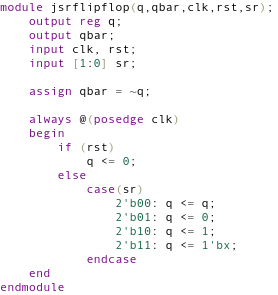
\includegraphics[width=6cm]{res/verilog.png}
			\end{tabular}
			
			& \begin{tabular}{l}
				\parbox{0.5\linewidth}{\scriptsize
					\begin{itemize}
						\item Each gate can be described with \textbf{hardware description language (HDL)}, like \textbf{Verilog} or \textbf{VHDL}.
						\item \textbf{Wires \& vias} can also be described.
						\item That's all we need to \textbf{obtain the netlist}!
					\end{itemize}
					
					We can, from HDL, \textbf{simulate the extracted netlist} and \textbf{find incoherence} (\textit{example with gtkwave below}):
					
					\vspace{2mm}
					
					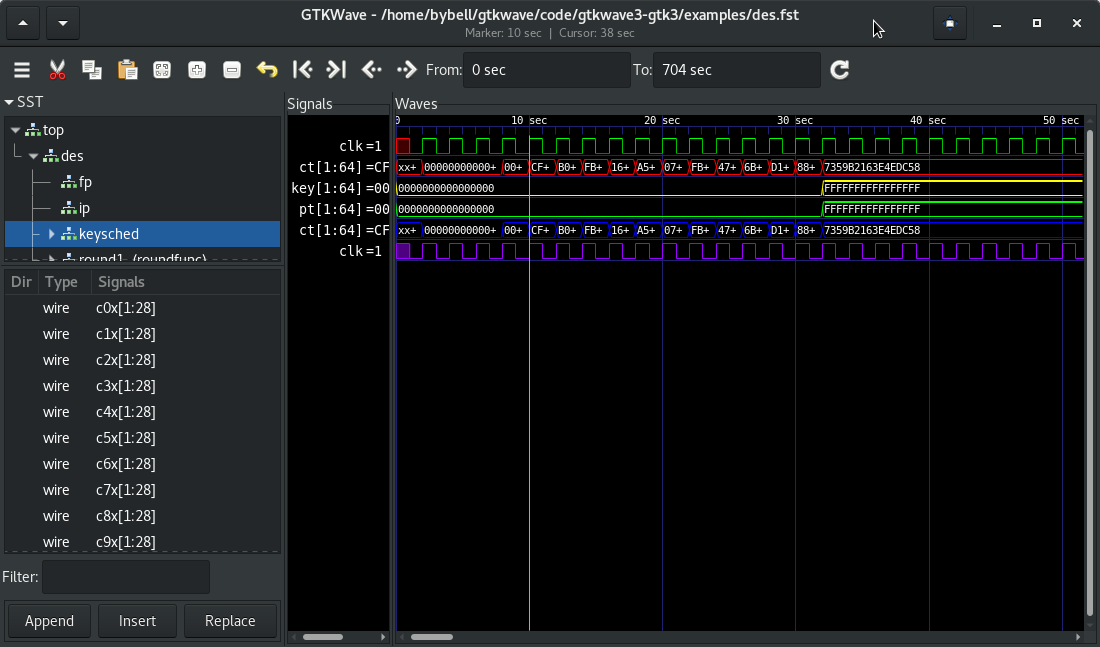
\includegraphics[width=7cm]{res/gtkwave.png}
				}
			\end{tabular}
			
		\end{tabular}
	\end{frame}
	%%%%%%%%%%%%%%%%%%%%%%%%%%%%%%%%%%%%%%%%%%%%%%%%%%
	
	%%%%%%%%%%%%%%%%%%%%%%%%%%%%%%%%%%%%%%%%%%%%%%%%%%
	\begin{frame}{How to Get the Algorithm/Specification from Netlist? \cite{LeonidAzriel2021}}
		\small
		
		After retrieving the \textbf{netlist}, we are left with a \textbf{huge and "unorganized" number of gates}. The \textbf{specification discovery} phase aims to \textbf{retrieve IC's algorithm/functionality} from the extracted netlist.
		
		\vspace{3mm}
		
		Using specific algorithms you can \textbf{automate some phase}:
		\begin{itemize}
			\item \textbf{Partitioning} of the netlist (\textit{to retrieve a semblance of "code" structure}).
			\item \textbf{Recovery} of the registers (\textit{if applicable}).
			\item \textbf{Identification} of the extracted "groups" (\textit{partitions}) of the netlist.
			\item \textbf{Construction} of a library of netlist components from the identified "groups".
		\end{itemize}
		
		\vspace{3mm}
		
		These algorithms \textbf{need to allow some degrees of error} from the netlist extraction. This phase is $\sim$analogous with \textbf{duplicated, standard \& library functions identification} for \textbf{software engineering}. A nice open source tool for this is \textbf{HAL}\footnote{https://github.com/emsec/hal} (compatible with Degate's outputs!).
	\end{frame}
	%%%%%%%%%%%%%%%%%%%%%%%%%%%%%%%%%%%%%%%%%%%%%%%%%%
	
	%%%%%%%%%%%%%%%%%%%%%%%%%%%%%%%%%%%%%%%%%%%%%%%%%%
	\begin{frame}{To Summarize}
		
		\begin{figure}[!ht]
			\centering
			\resizebox{0.8\textwidth}{!}{%
				\begin{tikzpicture}
					\tikzstyle{every node}=[font=\normalsize]
					\draw  (10.5,17.75) circle (2.5cm) node [text width=4cm]
					{ \Large
						\centering \textbf{Image chip} \\
						\vspace{3mm}
						\textit{(or SEM or 3D tomography)}
					} ;
					\draw  (16.5,17.75) circle (2.5cm) node {\Large \textbf{Analyze Gates}} ;
					\draw  (22.5,17.75) circle (2.5cm) node {\Large \textbf{Trace Wires/Vias}} ;
					\draw  (28.5,17.75) circle (2.5cm) node {\Large \textbf{Generate Netlist}} ;
					\draw [, dashed] (34.5,17.75) circle (2.5cm) node {\Large \textbf{Retrieve Algorithm}} ;
					\draw [->] (13,17.75) -- (14,17.75);
					\draw [->] (19,17.75) -- (20,17.75);
					\draw [->] (25,17.75) -- (26,17.75);
					\draw [->] (31,17.75) -- (32,17.75);
					
					\draw [, dashed] (8.25,15) rectangle  node [text width=4cm] 
					{ 
						- \textbf{Decapsulate}, \\
						- Select \textbf{area of interest}, \\
						- \textbf{Delayer}, \\
						- Clean, \\
						- Stitch.
					}  (12.75,10.25);
					
					\draw [, dashed] (14.25,15) rectangle  node [text width=4cm]
					{ 
						- Analyze transistors, \\
						- \textbf{Identify each type of gates}, \\
						- Retrieve all instances of each gate (\textbf{pattern matching}).
					}  (18.75,10.25);
					
					\draw [, dashed] (20.25,15) rectangle  node [text width=4cm]
					{
						- Identify \textbf{wires}, \\
						- Identify \textbf{vias}, \\
						- \textbf{Connect gates}.
					}  (24.75,10.25);
					
					\draw [, dashed] (26.25,15) rectangle  node [text width=4cm]
					{ 
						- \textbf{Export netlist}, \\
						- Gate simulation, \\
						- Try to identify errors.
					}  (30.75,10.25);
					
					\draw [, dashed] (32.25,15) rectangle  node [text width=4cm]
					{
						- Extract algorithm, \\
						- \textbf{Discover specification}, \\
						- Perform functional analysis\cite{LeonidAzriel2021}, \\
						- Build a \textbf{software emulator}, \\
						- Try to \textbf{identify errors}.
					}  (36.75,10.25);
					
					\draw [] (10.5,15.25) -- (10.5,15);
					\draw [] (16.5,15.25) -- (16.5,15);
					\draw [] (22.5,15.25) -- (22.5,15);
					\draw [] (28.5,15.25) -- (28.5,15);
					\draw [] (34.5,15.25) -- (34.5,15);
					

					\node (tikzmaker) [shift={(2.75, -0)}] at (7.5,7.25) {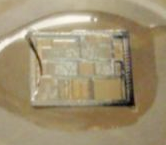
\includegraphics[width=5cm]{res/how_1.png}\cite{KarstenNohl2009}};
					\node (tikzmaker) [shift={(2.75, -0)}] at (13.5,7.25) {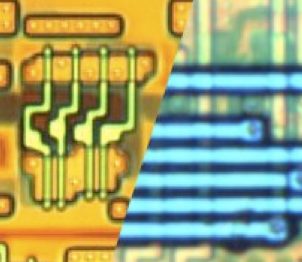
\includegraphics[width=5cm]{res/how_2.png}\cite{KarstenNohl2009}};
					\node (tikzmaker) [shift={(2.75, -0)}] at (19.5,6.5) {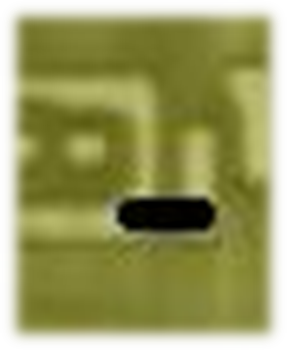
\includegraphics[width=5cm]{res/how_3.png}\cite{KarstenNohl2009}};
					\node (tikzmaker) [shift={(2.75, -0)}] at (25.5,7.25) {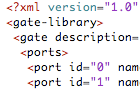
\includegraphics[width=5cm]{res/how_4.png}\cite{KarstenNohl2009}};
					\node (tikzmaker) [shift={(2.75, -0)}] at (31.75,7.25) {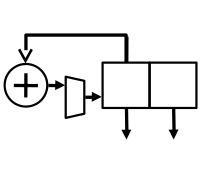
\includegraphics[width=5cm]{res/how_5.png}\cite{KarstenNohl2009}};
					
					\draw [, dashed] (10.25,10.25) -- (10.25,9.75);
					\draw [, dashed] (16.25,10.25) -- (16.25,9.75);
					\draw [, dashed] (22.25,10.25) -- (22.25,9.75);
					\draw [, dashed] (28.5,10.25) -- (28.5,9.75);
					\draw [, dashed] (34.5,10.25) -- (34.5,9.75);
				\end{tikzpicture}
			}%
		\end{figure}
	\end{frame}
	%%%%%%%%%%%%%%%%%%%%%%%%%%%%%%%%%%%%%%%%%%%%%%%%%%
	
%%%%%%%%%%%%%%%%%%%%%%%%%%%%%%%%%%%%%%%%%%%%%%%%%%%%%%%%%%%%%%%%%%%%%%%%%%%%%%%%

	\subsection{Challenges}
	
	%%%%%%%%%%%%%%%%%%%%%%%%%%%%%%%%%%%%%%%%%%%%%%%%%%
	
	\begin{frame}{}
		\tableofcontents[currentsubsection]
	\end{frame}
		
	%%%%%%%%%%%%%%%%%%%%%%%%%%%%%%%%%%%%%%%%%%%%%%%%%%
	\begin{frame}{Cost Perspective (1/2)}
		\textbf{Costly solutions will give best results}, and sometime reduce the difficulty for analysis software:
		\begin{itemize}
			\item \textbf{Decapsulation/delayering:} plasma, laser, FIB ;
			\item \textbf{Imaging:} Scanning Electron Microscope (SEM), other electron microscope (TEM, STEM, LEEM, PEEM...) ;
			\item \textbf{3D modelization:} electron tomography (3D) ;
		\end{itemize}
		
		\vspace{3mm}
		
		Simpler methods rely on \textbf{mechanical \& chemical} decapsulation/delayering and \textbf{optical microscopes} to obtain \textbf{very-high resolution but imperfect images}. Using images is more challenging: \textbf{color channels}, \textbf{impurity/damage/dust}, \textbf{single dimension}, \textbf{stitching}, \textbf{resolution}, \textbf{laborious work}...
	\end{frame}
	%%%%%%%%%%%%%%%%%%%%%%%%%%%%%%%%%%%%%%%%%%%%%%%%%%
	
	%%%%%%%%%%%%%%%%%%%%%%%%%%%%%%%%%%%%%%%%%%%%%%%%%%
	\begin{frame}{Cost Perspective (2/2)}
		\textbf{Chip samples cost} are also to consider (when doing invasive analysis, you'll maybe need multiple samples of the chip).
		
		\vspace{3mm}
		
		Compared to software reverse engineering, there is a \textbf{lot more costs associated}, and a \textbf{higher entry barrier}.
		
		\vspace{3mm}
		
		\begin{tabular}{cl}  
		
			\begin{tabular}{c}
				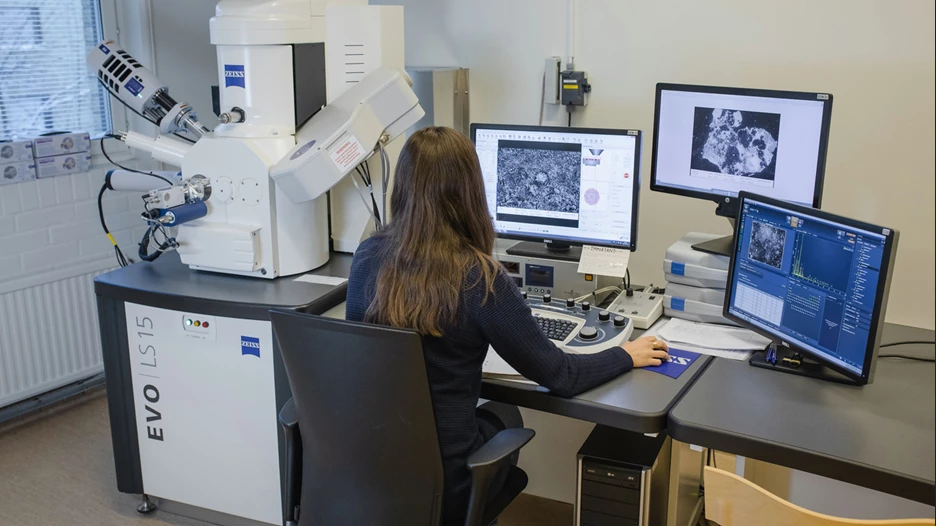
\includegraphics[width=7.5cm]{res/sem.png}
			\end{tabular}
			
			& \begin{tabular}{l}
				\parbox{0.4\linewidth}{\small
					A \textbf{new SEM microscope} can cost from \textbf{70k\$ to over 1M\$}. \textbf{Used instruments} can cost from \textbf{2,5k\$ to 550k\$}. Resolution may vary a lot. \\
					
					And that's \textbf{just for imaging}!
					
					\vspace{12mm}
					
					\textit{(Umeå University)}
				}
			\end{tabular}
			
		\end{tabular}
	\end{frame}
	%%%%%%%%%%%%%%%%%%%%%%%%%%%%%%%%%%%%%%%%%%%%%%%%%%
	
	%%%%%%%%%%%%%%%%%%%%%%%%%%%%%%%%%%%%%%%%%%%%%%%%%%
	\begin{frame}{Analysis Perspective}
		\begin{itemize}
			\item Newest chips \textbf{have $\sim$3nm transistors} and \textbf{billions of them}!
			\item Need automatic \textbf{gate recognition, wire tracing and netlist reconstruction}, which a human can't handle alone.
			\item Resulting images can be \textbf{millions of pixels large} ($width$ $>$ million pixels)!
			\item How to perform \textbf{template matching/image recognition} on such \textbf{gigantic images}?
			\item How to handle \textbf{all possible formats} (images, multi-layered images, SEM images, 3D tomography...)?
			\item There are so \textbf{many steps where that can go wrong}, or a \textbf{small error slips} into the analysis...
			\item Non-planerized IC exists (non repeated standard cells)! 
			\item And what about \textbf{obfuscation}? 
		\end{itemize}
	\end{frame}
	%%%%%%%%%%%%%%%%%%%%%%%%%%%%%%%%%%%%%%%%%%%%%%%%%%
	
	%%%%%%%%%%%%%%%%%%%%%%%%%%%%%%%%%%%%%%%%%%%%%%%%%%
	\begin{frame}{Human Perspective}		
		\begin{itemize}
			\item Need a \textbf{highly technical level} in several disciplines, this will help for \textbf{error spotting}, choosing a \textbf{zone of interest} and more.
			\item Need to \textbf{understand "silicon"} (how IC are made) and have \textbf{low-level electronic knowledge}.
			\item Have the necessary \\ \textbf{equipment available}.
			\item Be \textbf{persistent} and \textbf{patient}.
			\item \textbf{Practice}.
			\item And \textbf{Have time!}
		\end{itemize}
		
		\vspace{-30mm}
		\hfill\parbox{.65\textwidth}{
			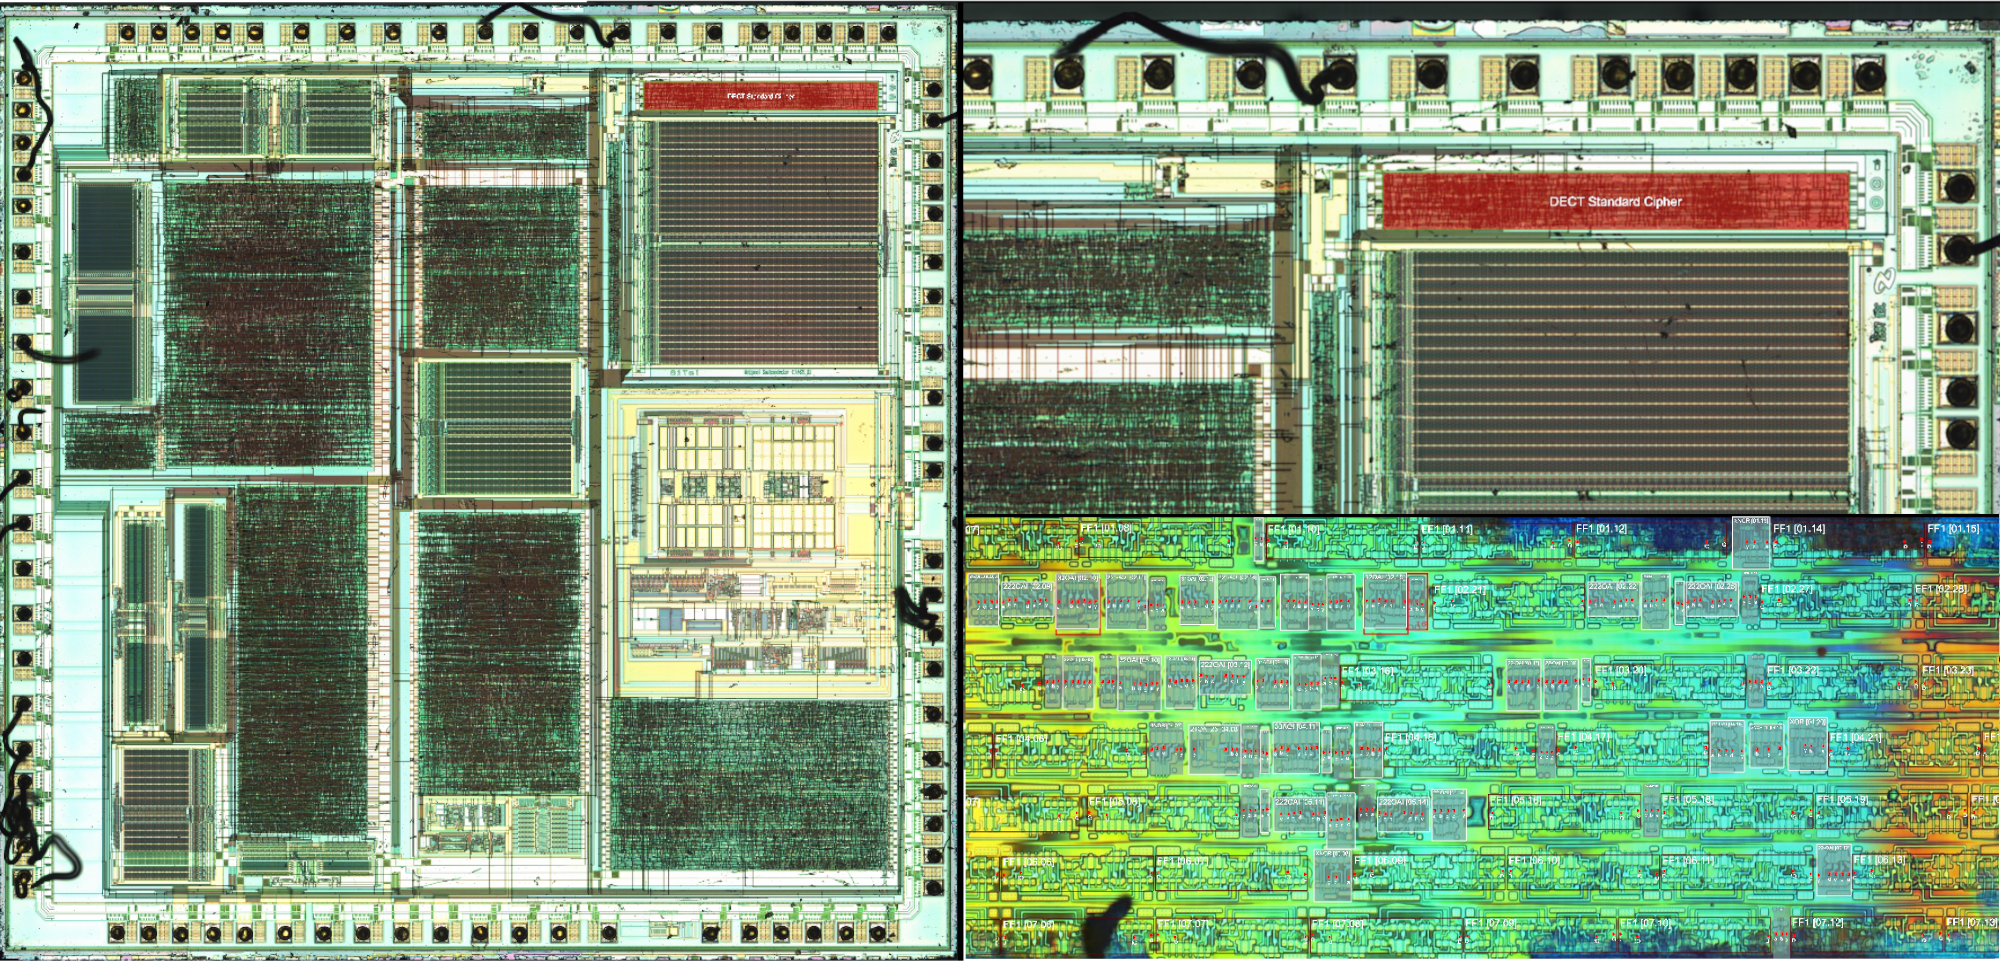
\includegraphics[width=9cm]{res/dect.png}
		}
	\end{frame}
	%%%%%%%%%%%%%%%%%%%%%%%%%%%%%%%%%%%%%%%%%%%%%%%%%%
	
	%%%%%%%%%%%%%%%%%%%%%%%%%%%%%%%%%%%%%%%%%%%%%%%%%%
	\begin{frame}{Importance for Cybersecurity}
		
		How can we \textbf{trust software} if we \textbf{can't trust hardware} (e.g. "specialized" ASIC)?
		
		\vspace{3mm}
		
		\begin{itemize}
			\item Is there any \textbf{vulnerability in the hardware implementation} of an algorithm (e.g. crypto standard with predictable initialization, bad randomness...)?
			\item Is there any \textbf{hardware Trojan} (e.g. placed by the foundry)?
			\item If there is a vulnerability/backdoor, \textbf{patching is impossible}, far \textbf{more impactful} than software vulnerabilities.
		\end{itemize}
		
		\vspace{3mm}
		
		Some examples of vulnerabilities found thanks to silicon RE:
		\begin{itemize}
			\item \textit{Legic Prime}, \textit{NXP Hitag2}, \textit{DECT DSC}, \textit{CryptoRF}, \textit{Atmel CryptoMemory} \& \textit{NXP Mifare Crypto-1} ($\sim$2008, Nohl et al): \textbf{weak (or potentially weak) cryptographic ciphers}.
			\item Undisclosed ones?
		\end{itemize}
	\end{frame}
	%%%%%%%%%%%%%%%%%%%%%%%%%%%%%%%%%%%%%%%%%%%%%%%%%%
	
		
	%%%%%%%%%%%%%%%%%%%%%%%%%%%%%%%%%%%%%%%%%%%%%%%%%%
	\begin{frame}{Available Tools \& Products}
		
		\begin{tabular}{cl}  
			
			\begin{tabular}{c}
				\parbox{0.4\linewidth}{\small
					Commercial products:
					\begin{itemize}
						\item \href{https://www.texplained.com/about-us/chipjuice-software/}{\textbf{CHIPJUICE}}: 
						Extracting Data from Highly Encrypted ICs.
						\item \textit{Internal tools}: for sure, there is a lot of them.
					\end{itemize}
					
					\vspace{3mm}
					
					Open Source tools:
					\begin{itemize}
						\item \href{https://www.degate.org/}{\textbf{Degate}}
						\item \href{https://github.com/emu-russia/psxrev}{\textbf{psxrev}}: SONY PlayStation PCB/chips reverse engineering.
						\item \href{https://github.com/emu-russia/Deroute}{\textbf{Deroute}}: Tool for untangling wires.
						\item \href{https://github.com/galibert/dietools}{\textbf{dietools}}: Series of tools for die shot reverse-engineering. % from vectorization to netlist
					\end{itemize}
				}
			\end{tabular}
			
			& \begin{tabular}{c}
				\includegraphics[width=7cm]{res/chipjuice.jpg} \\
				\textit{\small(Texplained)}
			\end{tabular}
			
		\end{tabular}
	\end{frame}
	%%%%%%%%%%%%%%%%%%%%%%%%%%%%%%%%%%%%%%%%%%%%%%%%%%
	
%%%%%%%%%%%%%%%%%%%%%%%%%%%%%%%%%%%%%%%%%%%%%%%%%%%%%%%%%%%%%%%%%%%%%%%%%%%%%%%%

%%%%%%%%%%%%%%%%%%%%%%%%%%%%%%%%%%%%%%%%%%%%%%%%%%%%%%%%%%%%%%%%%%%%%%%%%%%%%%%%
%%%%%%%%%%%%%%%%%%%%%%%%%%%%%%%%%%%%%%%%%%%%%%%%%%%%%%%%%%%%%%%%%%%%%%%%%%%%%%%%
%%%%%%%%%%%%%%%%%%%%%%%%%%%%%%%%%%%%%%%%%%%%%%%%%%%%%%%%%%%%%%%%%%%%%%%%%%%%%%%%

\section{Degate}
		
	%%%%%%%%%%%%%%%%%%%%%%%%%%%%%%%%%%%%%%%%%%%%%%%%%%
	\begin{frame}{Introduction}
		\textbf{Degate} is a multi-platform software for semi-automatic \textbf{Very-Large-Scale Integration (VLSI) chips reverse engineering} of digital logic in chips.
		
		\vspace{3mm}
		
		\begin{tabular}{cl}  
			
			\begin{tabular}{c}
				\parbox{0.4\linewidth}{\small
					\begin{itemize}
						\item $\sim$70k LoC
						\item Supports Mac, Linux \& Windows,
						\item Qt based,
						\item Multi-language support,
						\item Gate definition,
						\item Gate template, via \& wire matching,
						\item Rule checks,
						\item ...
					\end{itemize}
				}
			\end{tabular}
			
			& \begin{tabular}{l}
				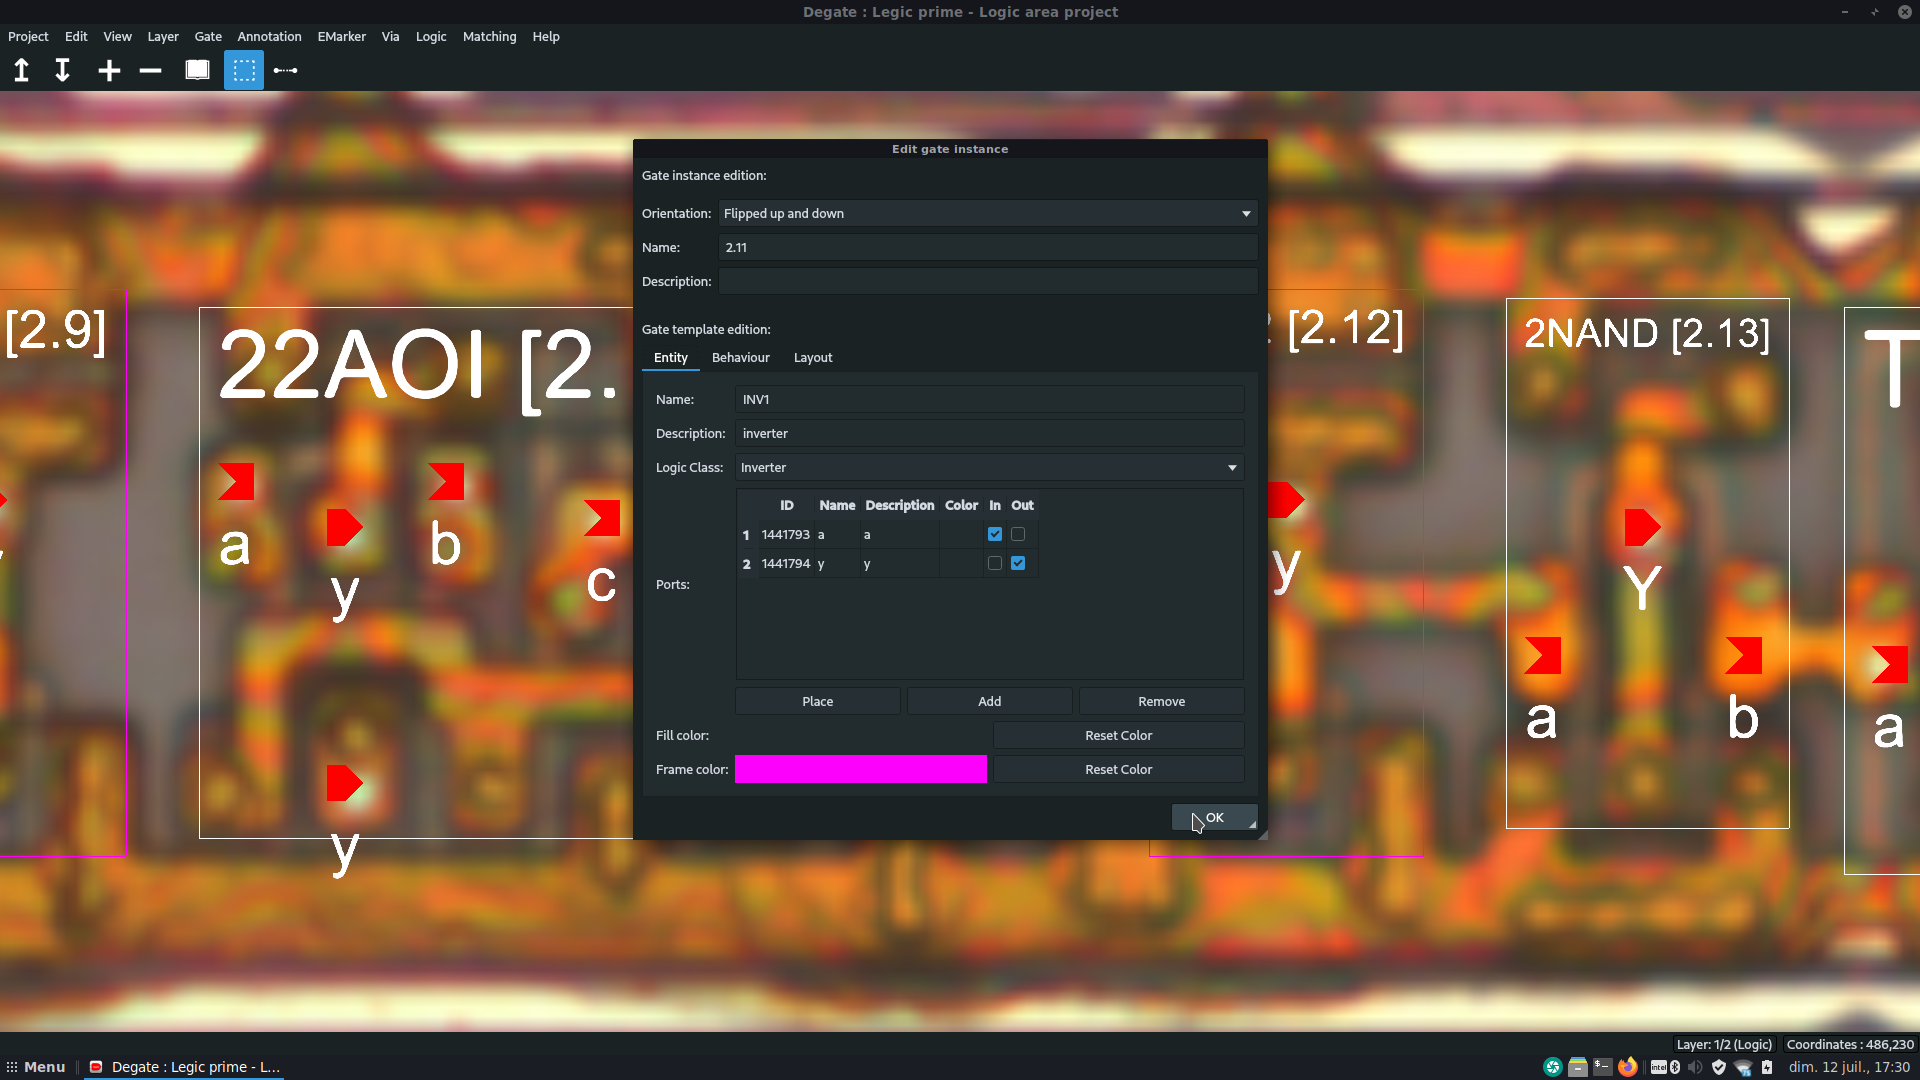
\includegraphics[width=7cm]{res/degate1.png}
			\end{tabular}
			
		\end{tabular}
	\end{frame}
	%%%%%%%%%%%%%%%%%%%%%%%%%%%%%%%%%%%%%%%%%%%%%%%%%%
	
		
	%%%%%%%%%%%%%%%%%%%%%%%%%%%%%%%%%%%%%%%%%%%%%%%%%%
	\begin{frame}{History}
		A long story, with \textbf{technical debt} and \textbf{major IC evolution} (in transistor count), along with a \textbf{small community}.
		
		\vspace{-10mm}
		
		\begin{center}
			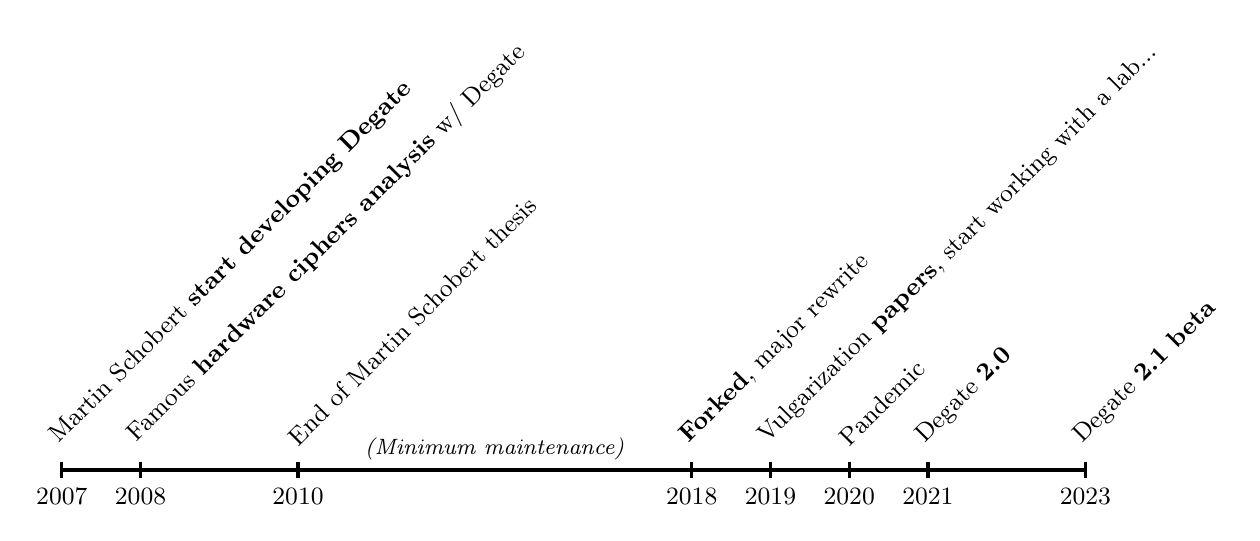
\begin{tikzpicture}[very thick, black, rotLabel/.style={above=3pt, anchor= south west, rotate=45}]
				\small
				
				% draw a horizontal line
				\draw (1,0) -- (14,0);
				
				% draw vertical lines
				\foreach \x in {1,2,4,9,10,11,12,14}
				\draw (\x cm,3pt) -- (\x cm,-3pt);
				
				% draw nodes to add events
				\draw (1,0) node[below=3pt] {2007} node[rotLabel] {Martin Schobert \textbf{start developing Degate}};
				\draw (2,0) node[below=3pt] {2008} node[rotLabel] {Famous \textbf{hardware ciphers analysis} w/ Degate};
				\draw (4,0) node[below=3pt] {2010} node[rotLabel] {End of Martin Schobert thesis};
				
				\draw (6.5,0) node[above=0pt] {\footnotesize \textit{(Minimum maintenance)}};
				
				\draw (9,0) node[below=3pt] {2018} node[rotLabel] {\textbf{Forked}, major rewrite};
				\draw (10,0) node[below=3pt] {2019} node[rotLabel] {Vulgarization \textbf{papers}, start working with a lab...};
				\draw (11,0) node[below=3pt] {2020} node[rotLabel] {Pandemic};
				\draw (12,0) node[below=3pt] {2021} node[rotLabel] {Degate \textbf{2.0}};
				\draw (14,0) node[below=3pt] {2023} node[rotLabel] {Degate \textbf{2.1 beta}};
			\end{tikzpicture}
		\end{center}
	\end{frame}
	%%%%%%%%%%%%%%%%%%%%%%%%%%%%%%%%%%%%%%%%%%%%%%%%%%
	
	%%%%%%%%%%%%%%%%%%%%%%%%%%%%%%%%%%%%%%%%%%%%%%%%%%
	\begin{frame}{Usage}
		
		Degate help to reverse \textbf{VLSI chips} by creating an analyzed \textbf{gate library}, doing \textbf{template matching} to find gates instances from this library, \textbf{matching wires \& vias}, \textbf{exporting netlist} and \textbf{navigating really huge images}. \\
		
		\vspace{3mm}
		
		Focus on \textbf{modern ICs} with \textbf{standard cells}, and supports \textbf{any 2D capture/imaging method} (SEM, optical...).
		
		\begin{figure}[!ht]
			\centering
			\resizebox{0.7\textwidth}{!}{%
				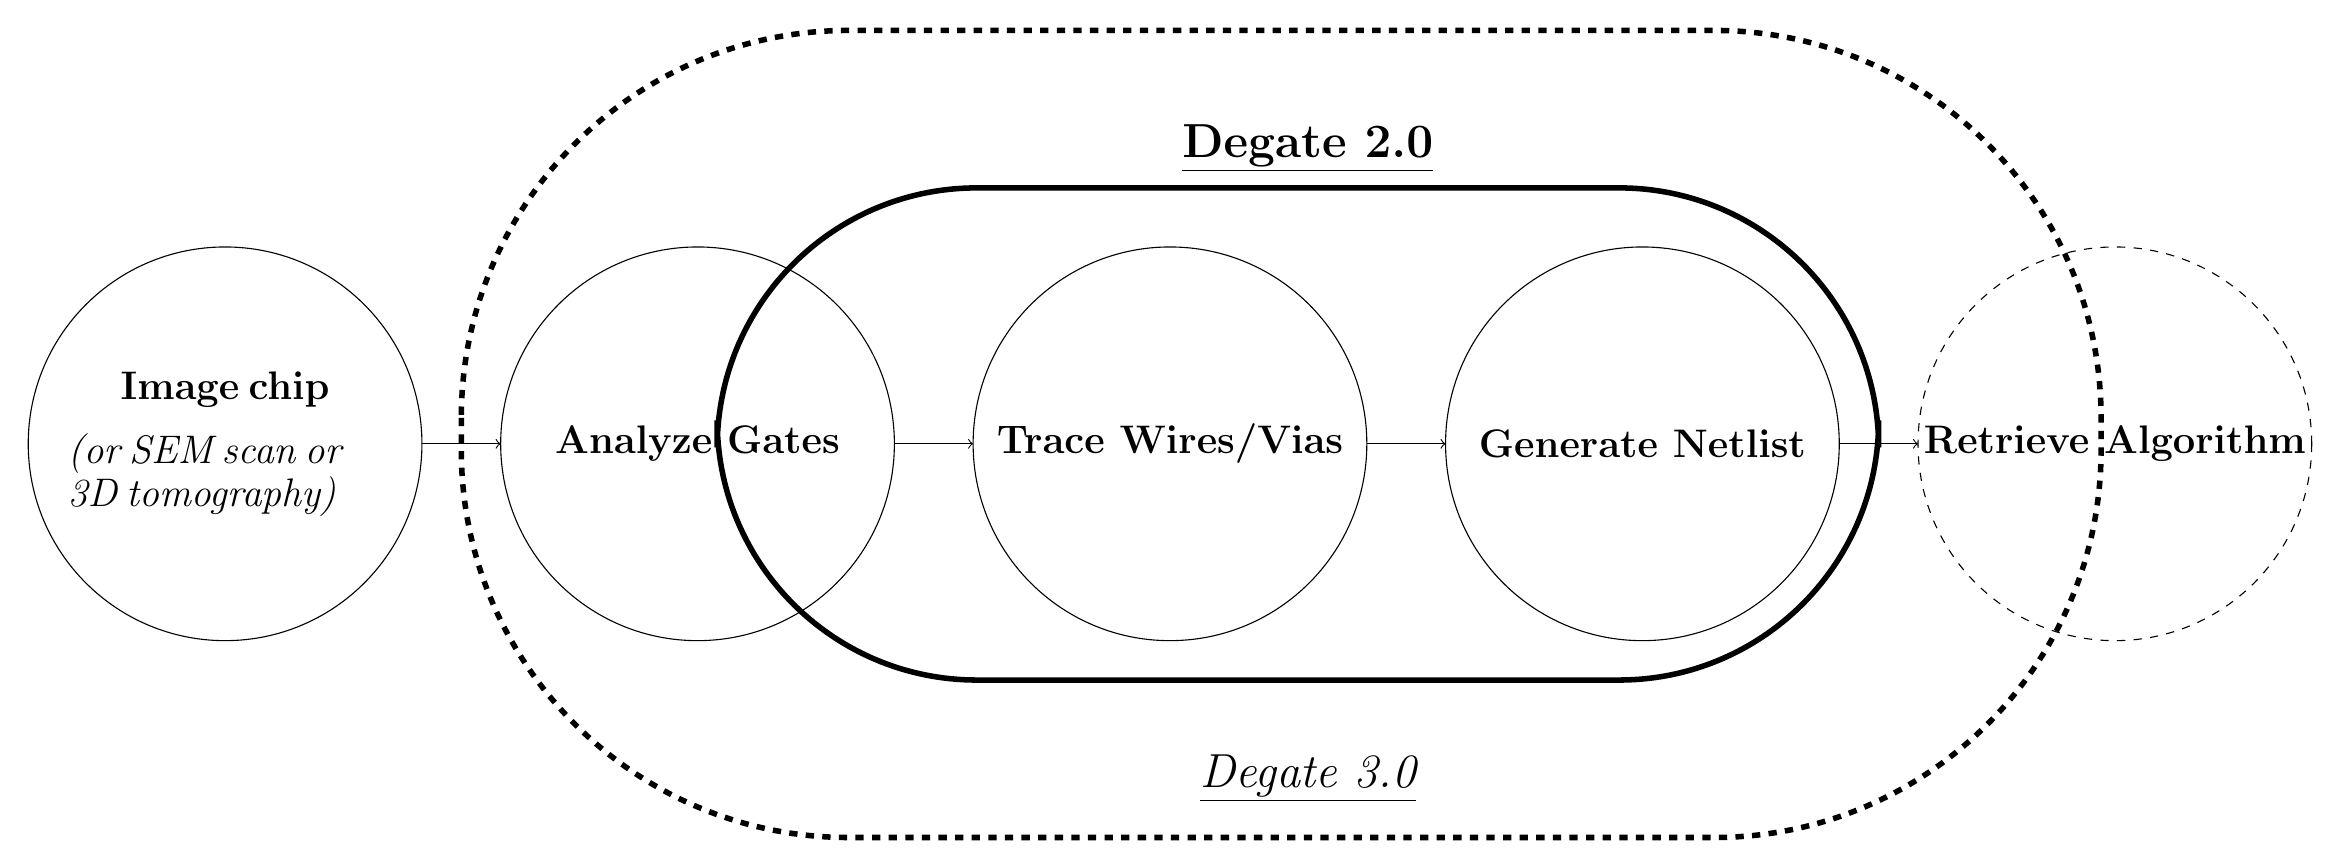
\begin{tikzpicture}
					\tikzstyle{every node}=[font=\normalsize]
					
					\draw [, line width=2pt, rounded corners = 93.8] (16.75,21) rectangle (31.5,14.75); % 16.75 -> 14.5
					\node [font=\LARGE] at (24.25,21.5) {\textbf{\underline{Degate 2.0}}}; % 24.25 -> 22.5
					
					\draw [dashed, line width=2pt, rounded corners = 140] (13.5,23) rectangle (34.325,12.75); % 16.75 -> 14.5
					\node [font=\LARGE] at (24.25,13.5) {\textit{\underline{Degate 3.0}}}; % 24.25 -> 22.5
						
					\draw  (10.5,17.75) circle (2.5cm) node [text width=4cm]
					{ \Large
						\centering \textbf{Image chip} \\
						\vspace{3mm}
						\textit{(or SEM scan or 3D tomography)}
					} ;
					\draw  (16.5,17.75) circle (2.5cm) node {\Large \textbf{Analyze Gates}} ;
					\draw  (22.5,17.75) circle (2.5cm) node {\Large \textbf{Trace Wires/Vias}} ;
					\draw  (28.5,17.75) circle (2.5cm) node {\Large \textbf{Generate Netlist}} ;
					\draw [, dashed] (34.5,17.75) circle (2.5cm) node {\Large \textbf{Retrieve Algorithm}} ;
					\draw [->] (13,17.75) -- (14,17.75);
					\draw [->] (19,17.75) -- (20,17.75);
					\draw [->] (25,17.75) -- (26,17.75);
					\draw [->] (31,17.75) -- (32,17.75);
				\end{tikzpicture}
			}%
		\end{figure}
	\end{frame}
	%%%%%%%%%%%%%%%%%%%%%%%%%%%%%%%%%%%%%%%%%%%%%%%%%%
	
	%%%%%%%%%%%%%%%%%%%%%%%%%%%%%%%%%%%%%%%%%%%%%%%%%%
	\begin{frame}{Small Demonstration}
		
		\begin{tabular}{cl}  
			
			\begin{tabular}{l}
				\hspace{-8mm}
				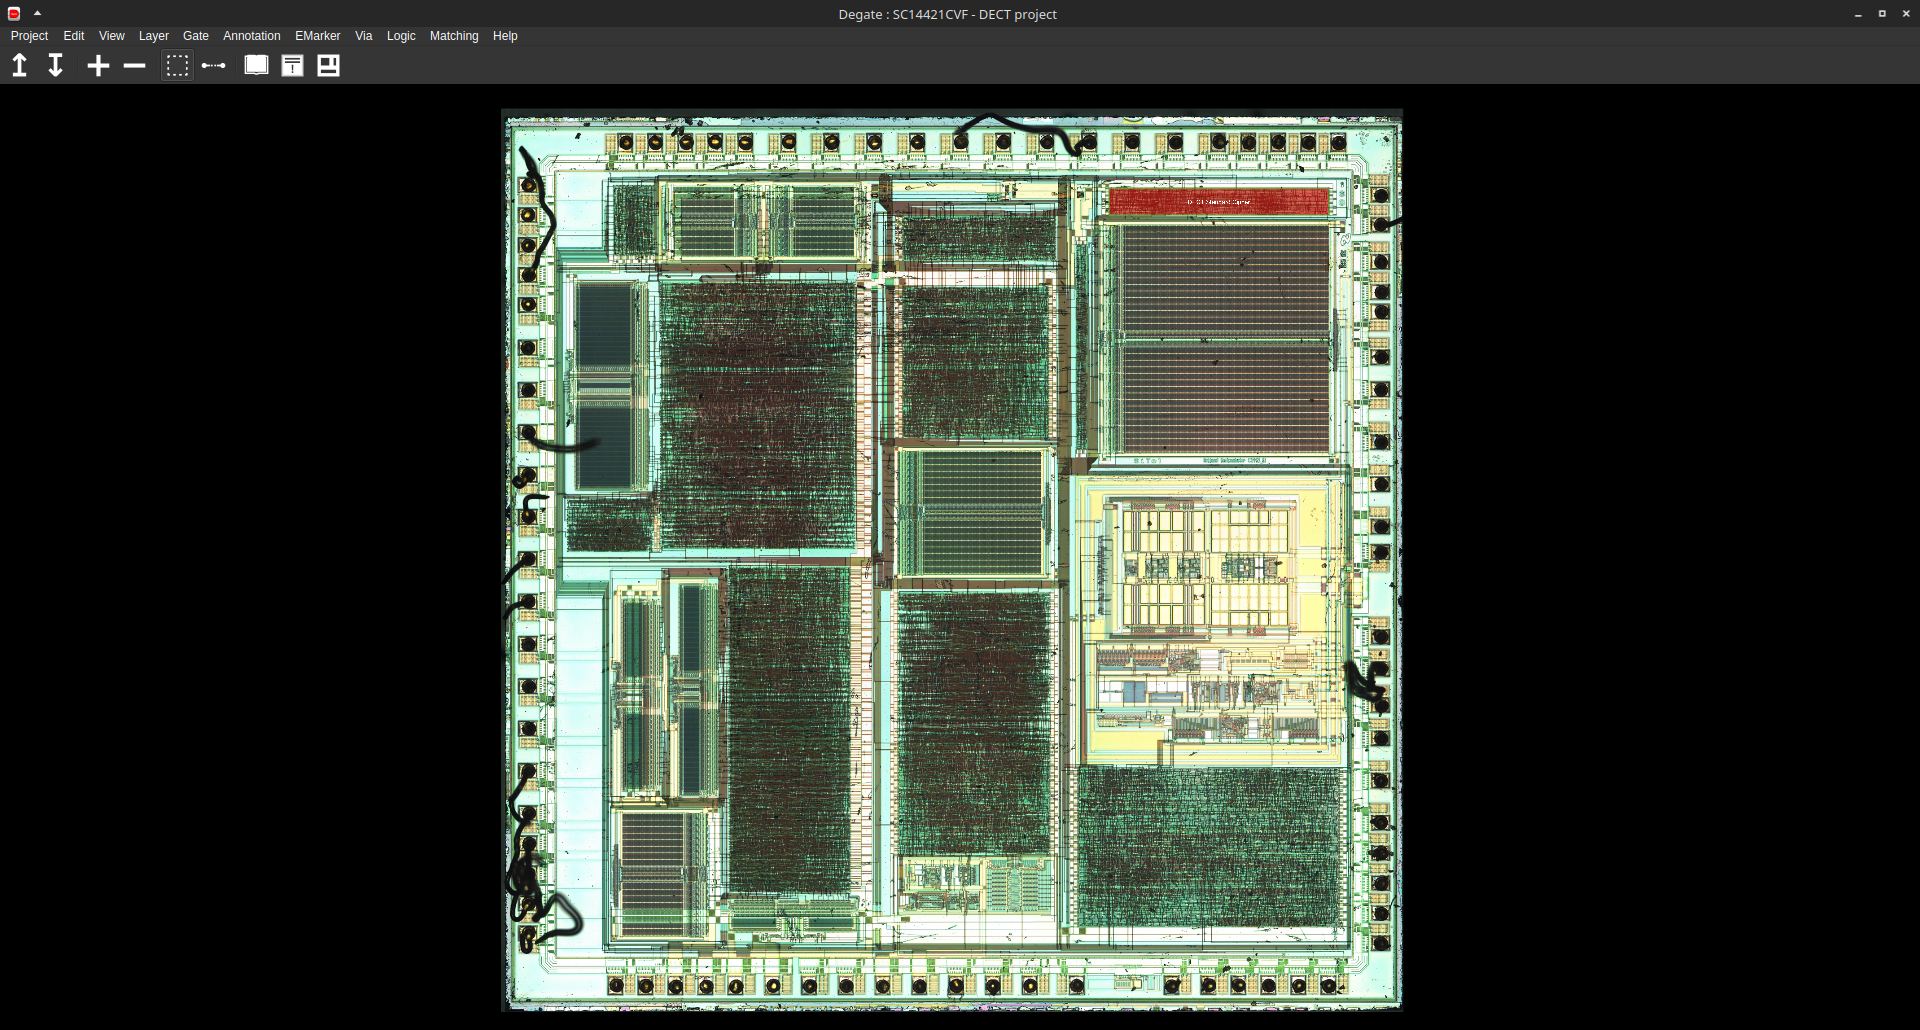
\includegraphics[width=0.8\textwidth]{res/degate_overview.png}
			\end{tabular}
		
			& 
				
			\begin{tabular}{l}
				\hspace{-8mm}
				\parbox{0.225\textwidth}{\footnotesize
					Overview of the chip, for zone of interest selection. \\
					
					A sub-project can then be created on the zone of interest, and specific layers can be added (independent from the rest).
				}
			\end{tabular}
		\end{tabular}
	\end{frame}
	%%%%%%%%%%%%%%%%%%%%%%%%%%%%%%%%%%%%%%%%%%%%%%%%%%
	
	%%%%%%%%%%%%%%%%%%%%%%%%%%%%%%%%%%%%%%%%%%%%%%%%%%
	\begin{frame}{Small Demonstration}
		
		\begin{tabular}{cl}  
			
			\begin{tabular}{l}
				\hspace{-8mm}
				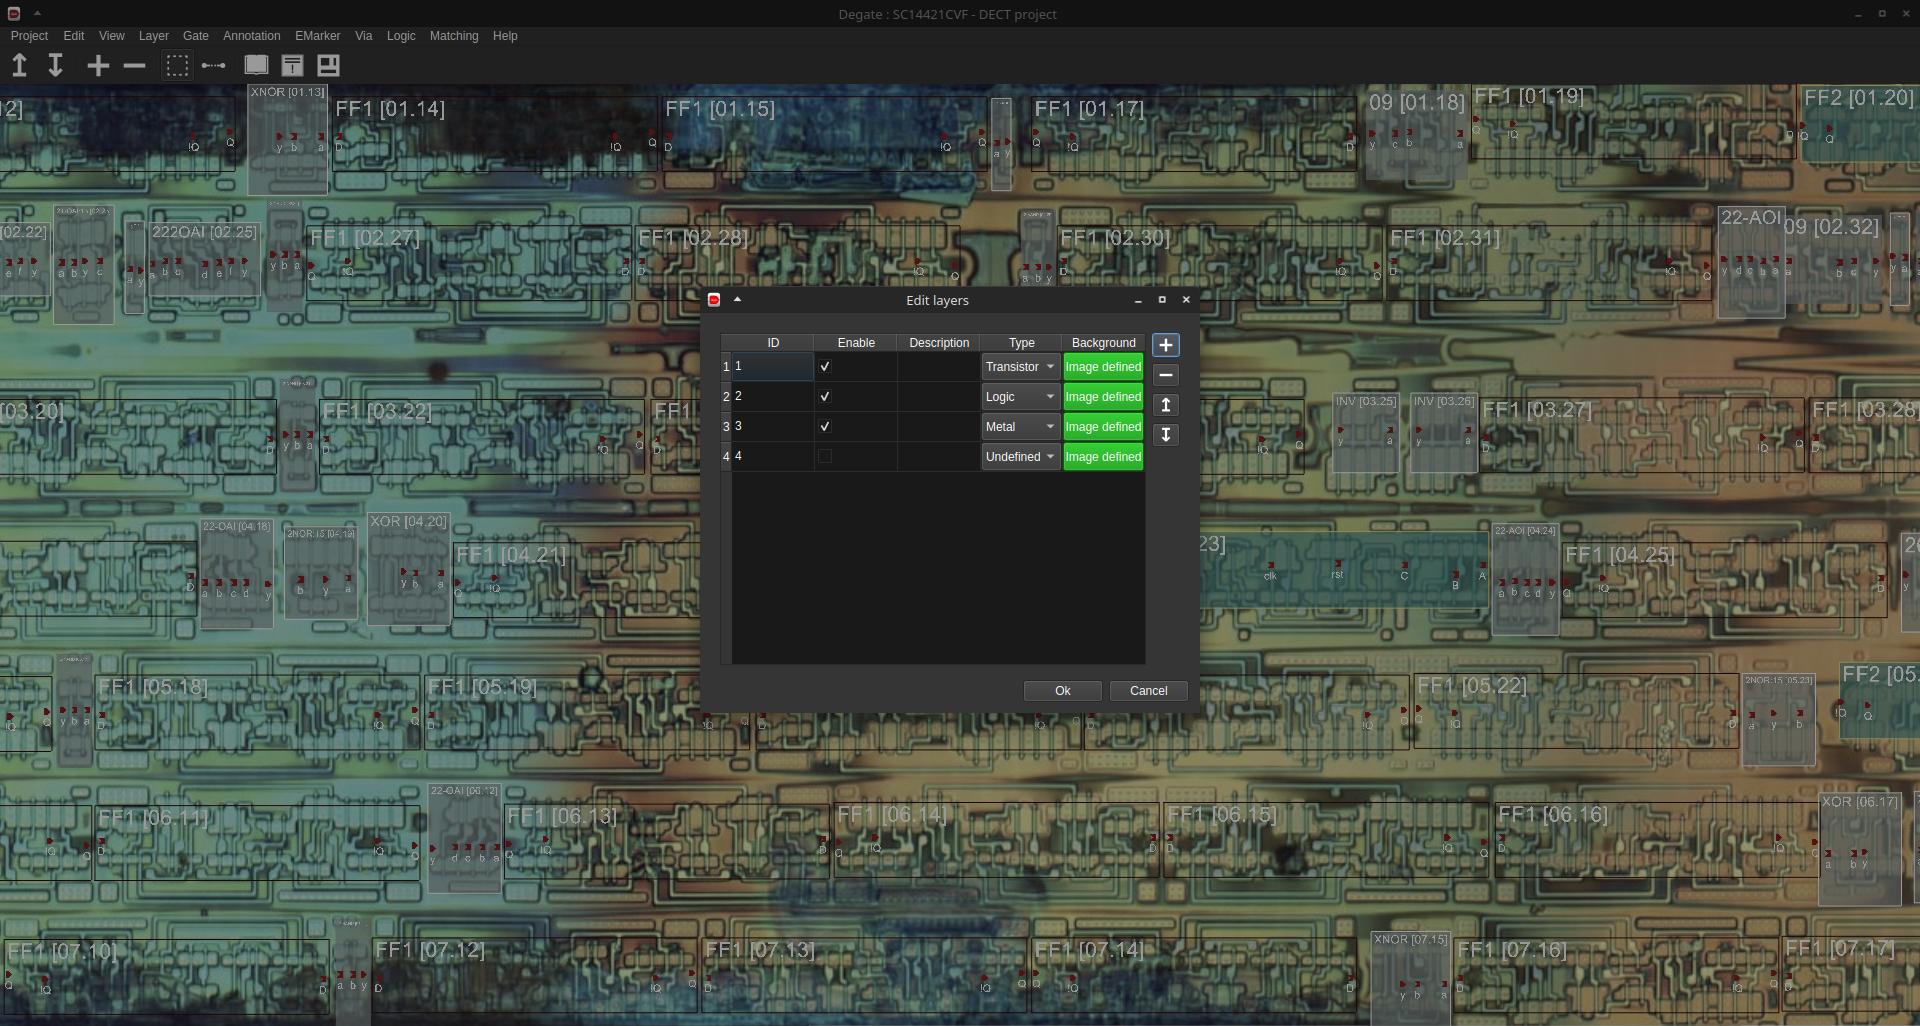
\includegraphics[width=0.8\textwidth]{res/degate_layers.png}
			\end{tabular}
			
			& 
			
			\begin{tabular}{l}
				\hspace{-8mm}
				\parbox{0.225\textwidth}{\footnotesize
					Each sub-project can contains multiple layers (pre-aligned images). \\
					
					Two project mode: 1. For smaller images, will convert each images in Degate's format (for fast access) and 2. New (WIP, beta) mode for huge images (load only partial tiles in RAM, and doesn't change/import initial file).
				}
			\end{tabular}
		\end{tabular}
	\end{frame}
	%%%%%%%%%%%%%%%%%%%%%%%%%%%%%%%%%%%%%%%%%%%%%%%%%%
	
	%%%%%%%%%%%%%%%%%%%%%%%%%%%%%%%%%%%%%%%%%%%%%%%%%%
	\begin{frame}{Small Demonstration}
		
		\begin{tabular}{cl}  
			
			\begin{tabular}{l}
				\hspace{-8mm}
				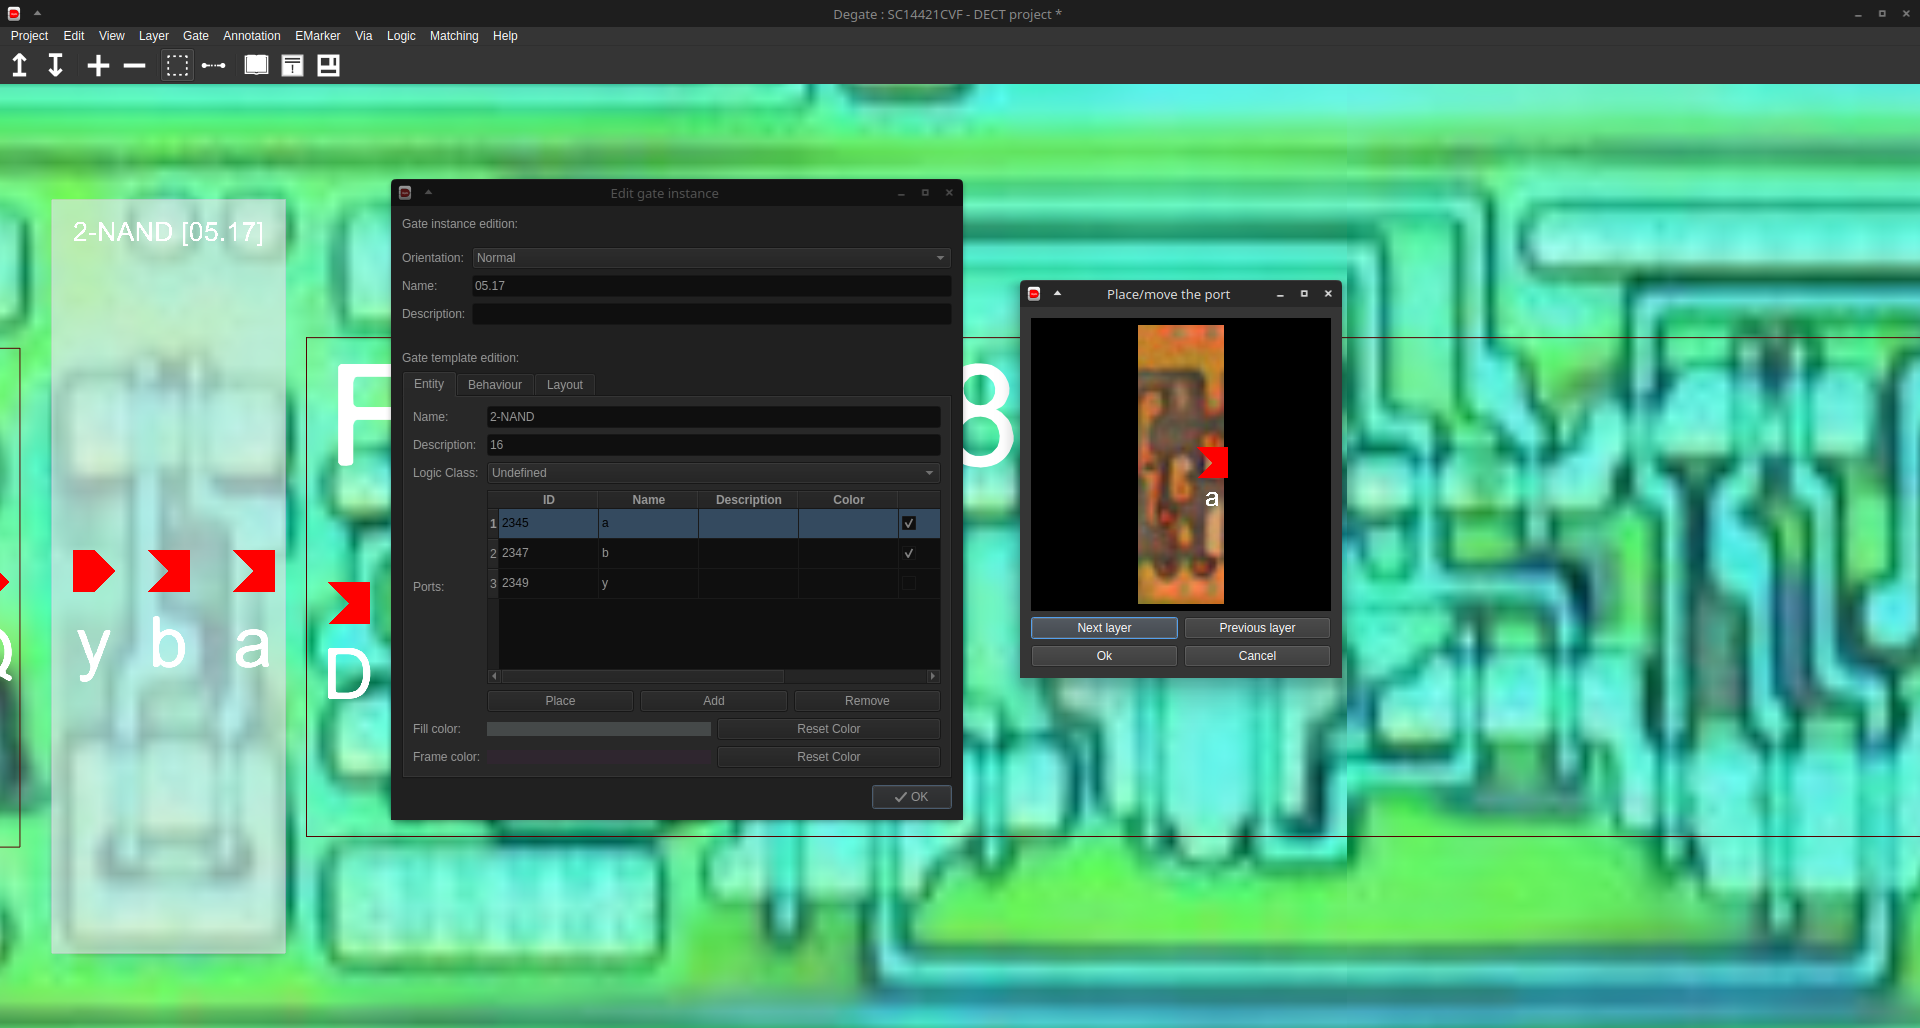
\includegraphics[width=0.8\textwidth]{res/degate_gate.png}
			\end{tabular}
			
			& 
			
			\begin{tabular}{l}
				\hspace{-8mm}
				\parbox{0.225\textwidth}{\footnotesize
					Each gate can be described with VHDL/Verilog, have a list of port (placed on image), a type associated etc.
				}
			\end{tabular}
		\end{tabular}
	\end{frame}
	%%%%%%%%%%%%%%%%%%%%%%%%%%%%%%%%%%%%%%%%%%%%%%%%%%
	
	%%%%%%%%%%%%%%%%%%%%%%%%%%%%%%%%%%%%%%%%%%%%%%%%%%
	\begin{frame}{Small Demonstration}
		
		\begin{tabular}{cl}  
			
			\begin{tabular}{l}
				\hspace{-8mm}
				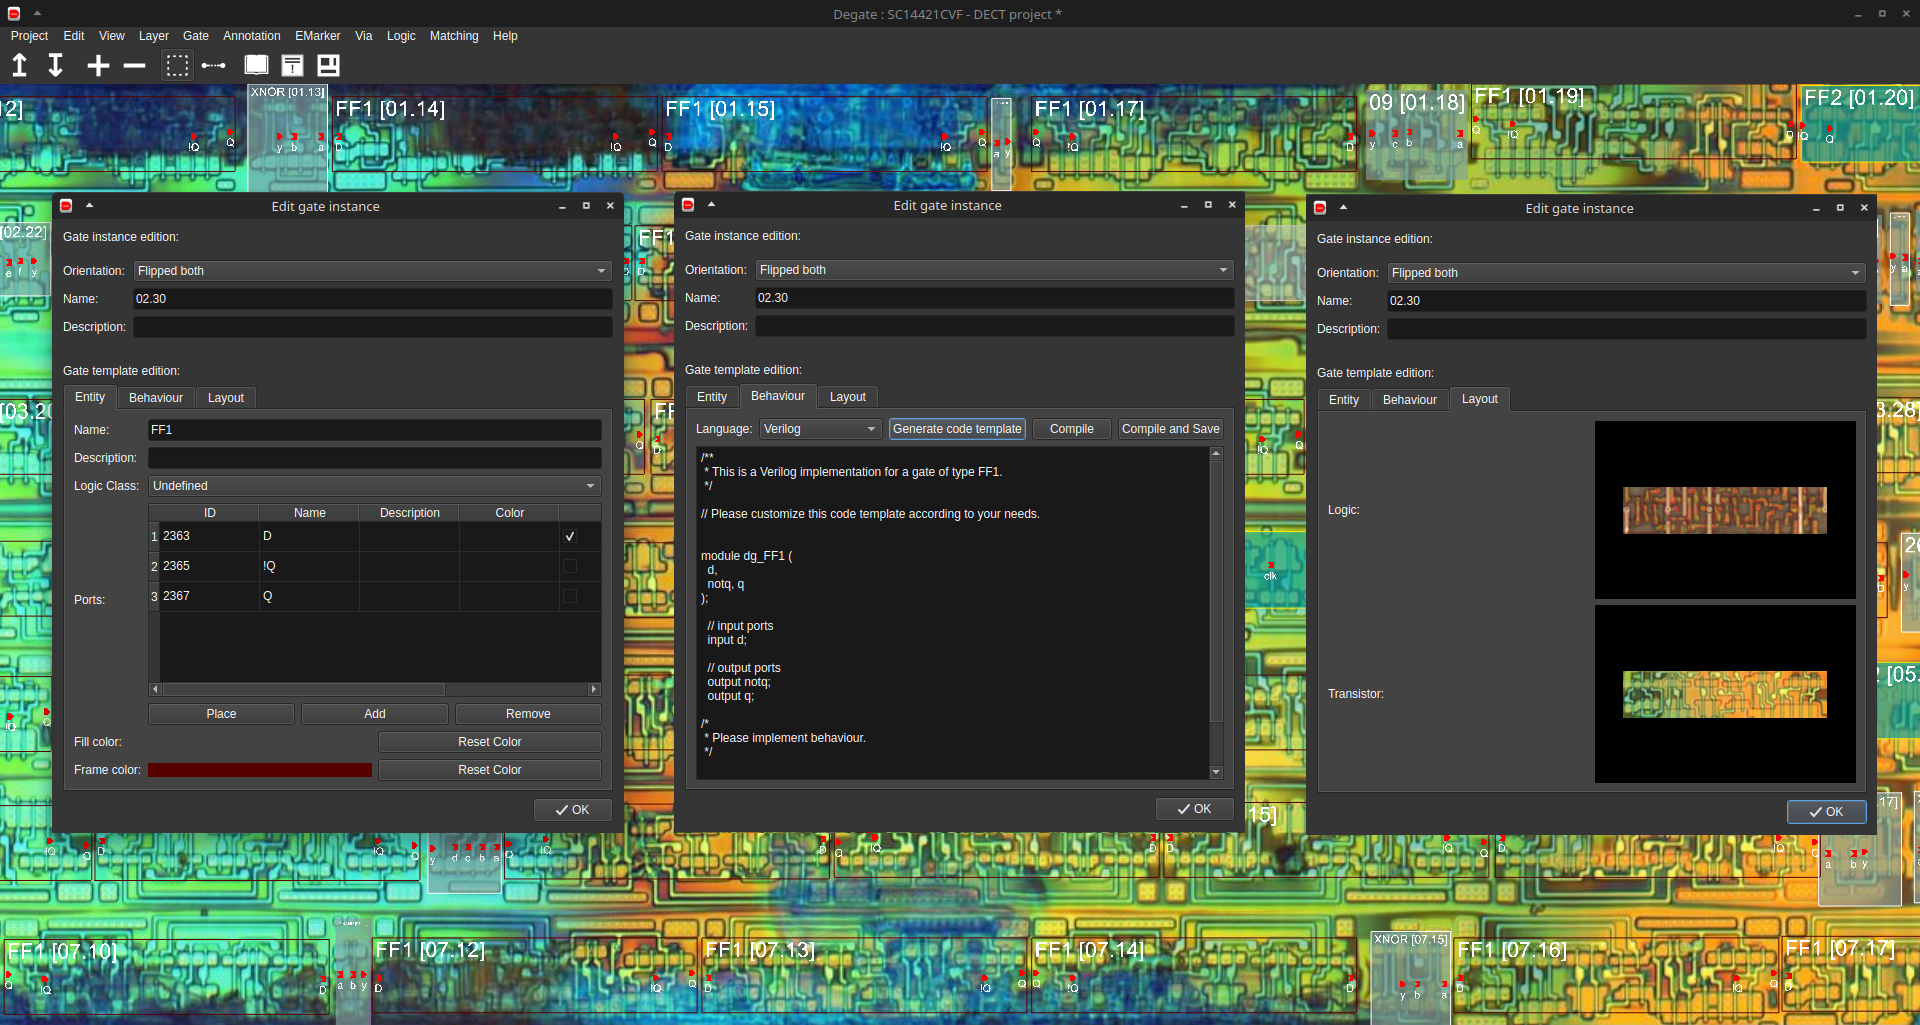
\includegraphics[width=0.8\textwidth]{res/degate_instance.png}
			\end{tabular}
			
			& 
			
			\begin{tabular}{l}
				\hspace{-8mm}
				\parbox{0.225\textwidth}{\footnotesize
					Each identified gate (from the gate library) can be matched manually or using template matching algorithms.
				}
			\end{tabular}
		\end{tabular}
	\end{frame}
	%%%%%%%%%%%%%%%%%%%%%%%%%%%%%%%%%%%%%%%%%%%%%%%%%%
	
	%%%%%%%%%%%%%%%%%%%%%%%%%%%%%%%%%%%%%%%%%%%%%%%%%%
	\begin{frame}{Small Demonstration}
		
		\begin{tabular}{cl}  
			
			\begin{tabular}{l}
				\hspace{-8mm}
				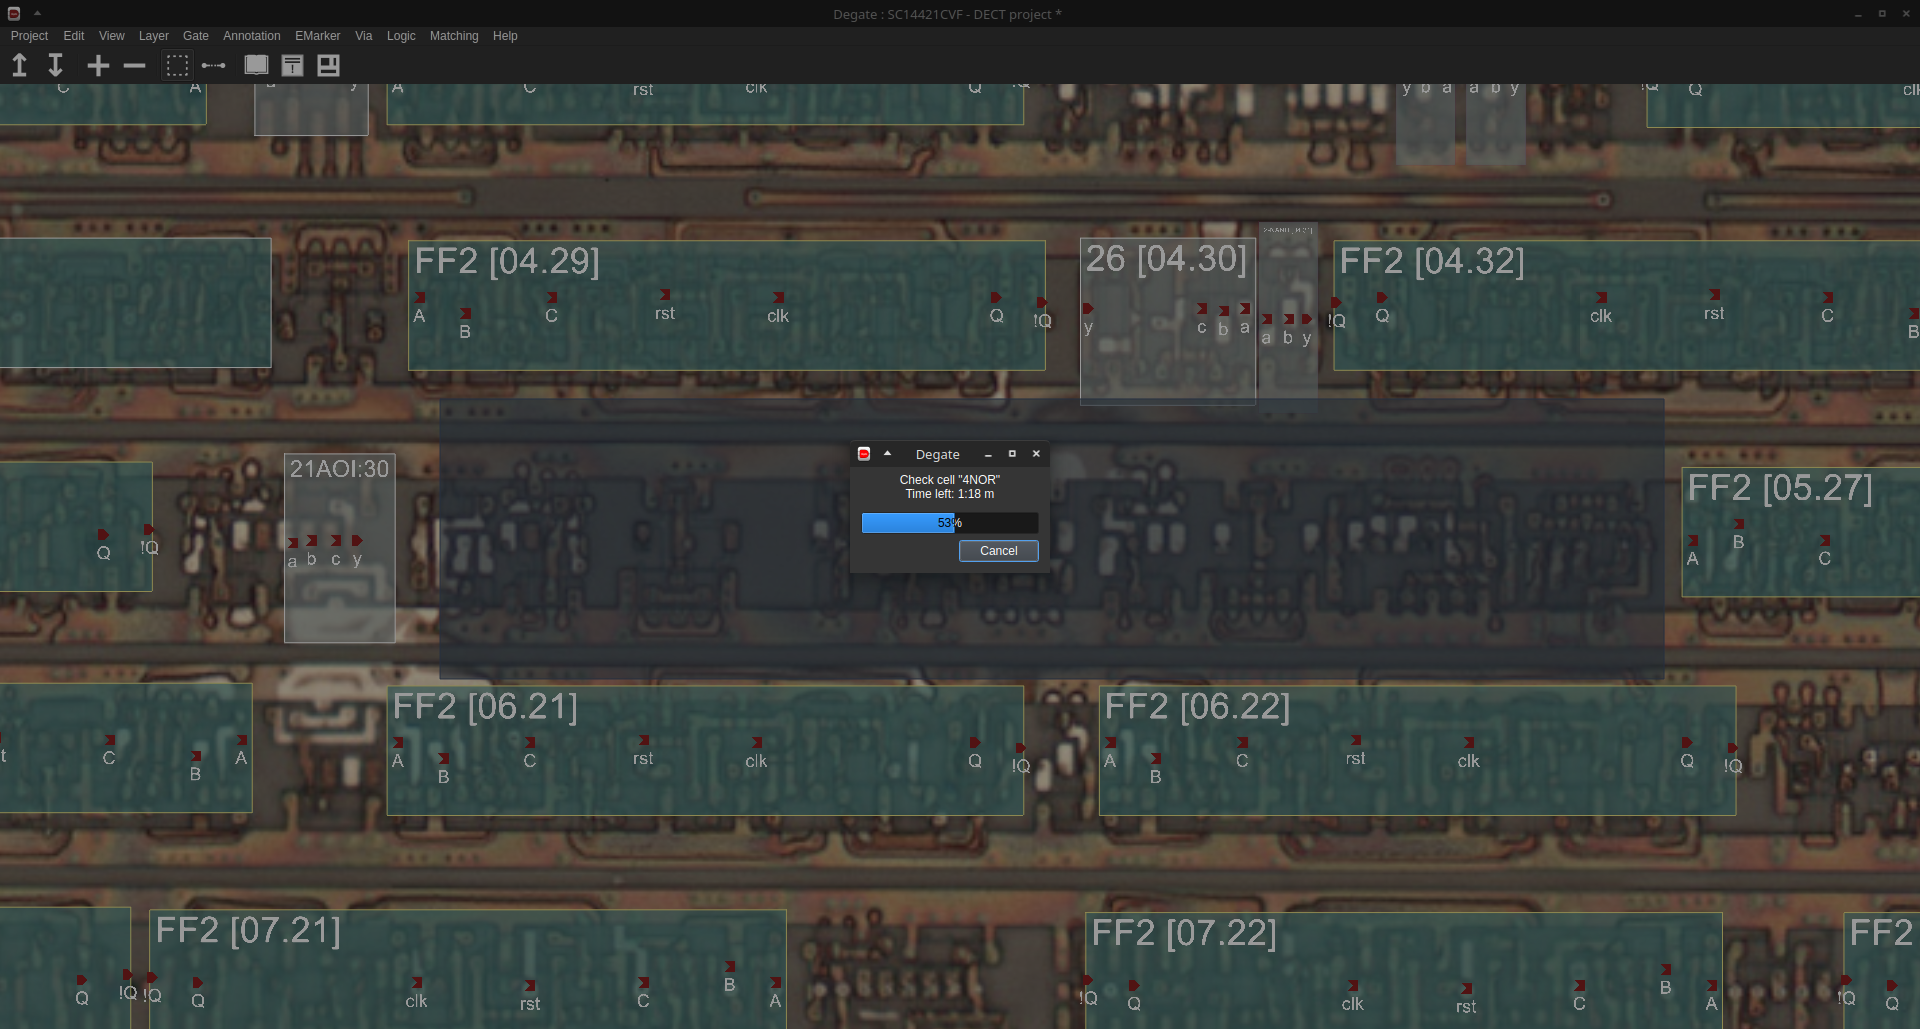
\includegraphics[width=0.8\textwidth]{res/degate_matching.png}
			\end{tabular}
			
			& 
			
			\begin{tabular}{l}
				\hspace{-8mm}
				\parbox{0.225\textwidth}{\footnotesize
					Template matching (will soon be ported to OpenCV) will use gate library to automate gate identification. \\
					
					Currently it uses normalized cross-correlation (with some more steps).
				}
			\end{tabular}
		\end{tabular}
	\end{frame}
	%%%%%%%%%%%%%%%%%%%%%%%%%%%%%%%%%%%%%%%%%%%%%%%%%%
	
	%%%%%%%%%%%%%%%%%%%%%%%%%%%%%%%%%%%%%%%%%%%%%%%%%%
	\begin{frame}{Small Demonstration}
		
		\begin{tabular}{cl}  
			
			\begin{tabular}{l}
				\hspace{-8mm}
				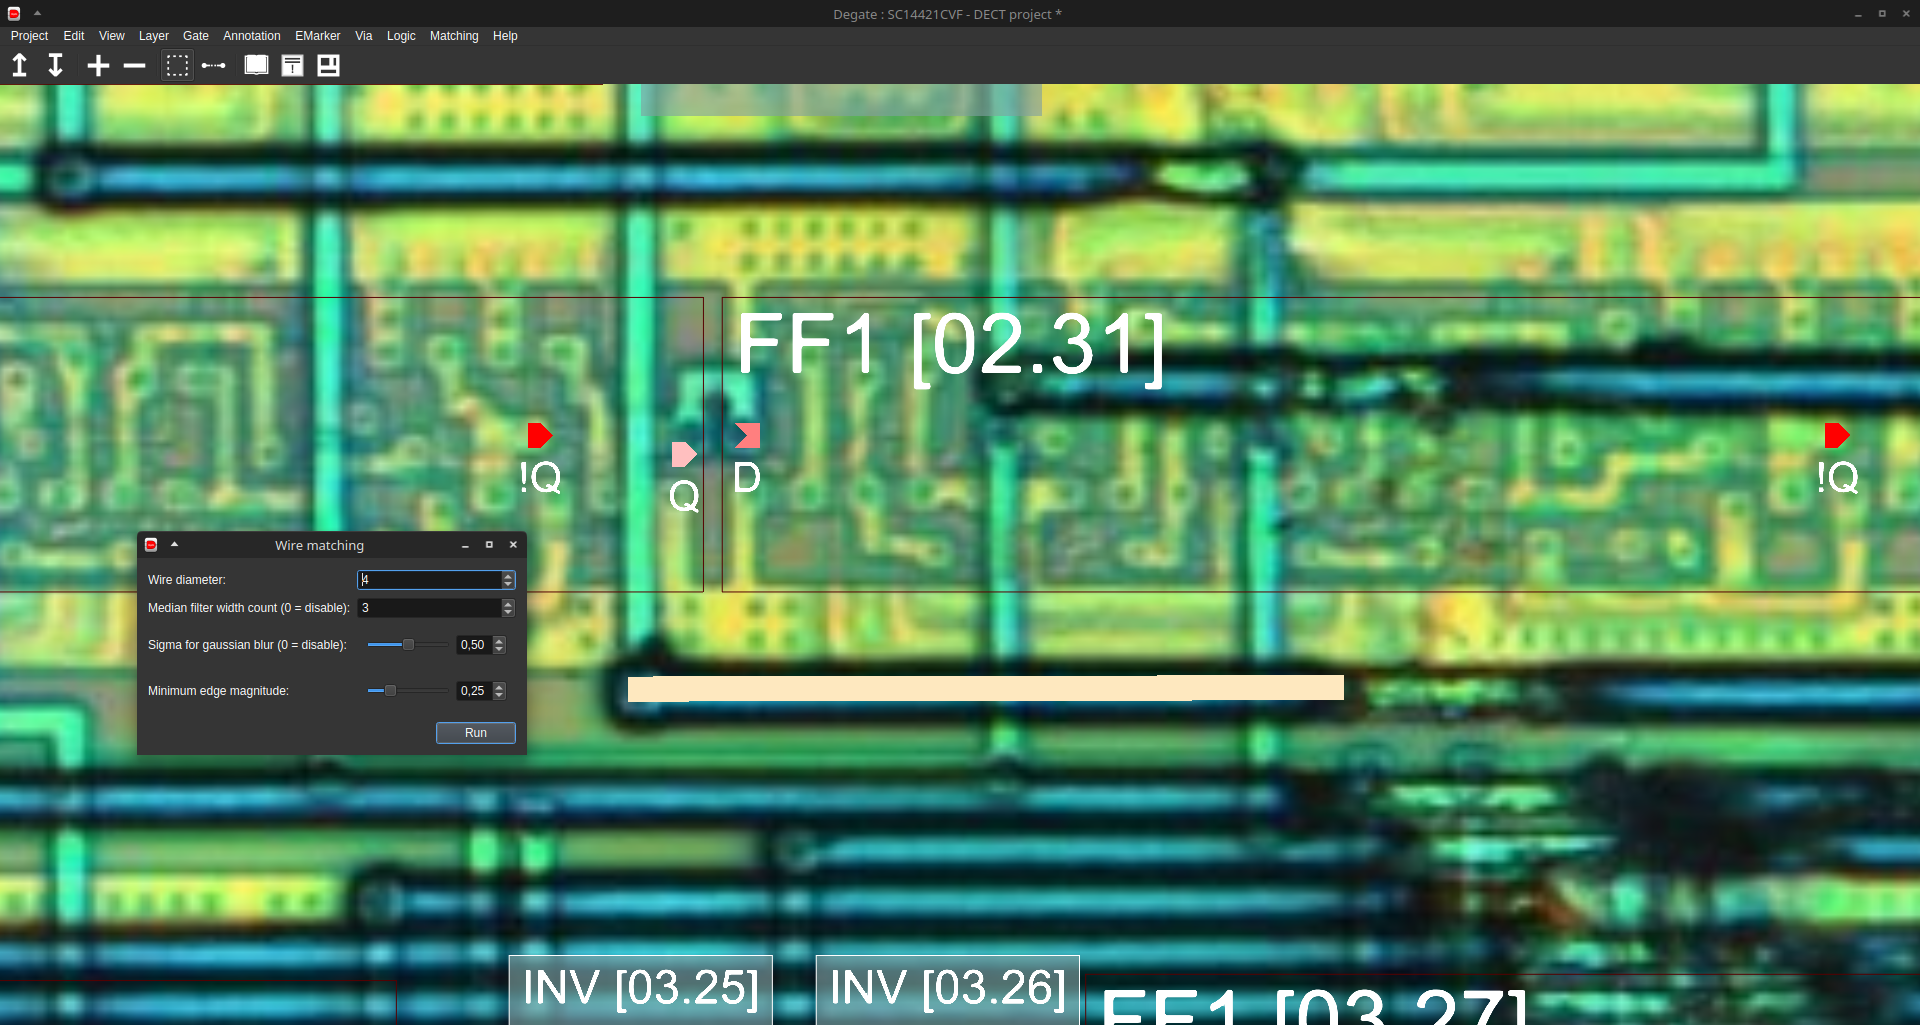
\includegraphics[width=0.8\textwidth]{res/degate_wires.png}
			\end{tabular}
			
			& 
			
			\begin{tabular}{l}
				\hspace{-8mm}
				\parbox{0.225\textwidth}{\footnotesize
					Wire matching, and specifically port interconnection, is the real challenge (and very error prone). \\
					
					Currently it uses zero crossing edge detection.
				}
			\end{tabular}
		\end{tabular}
	\end{frame}
	%%%%%%%%%%%%%%%%%%%%%%%%%%%%%%%%%%%%%%%%%%%%%%%%%%
	
	%%%%%%%%%%%%%%%%%%%%%%%%%%%%%%%%%%%%%%%%%%%%%%%%%%
	\begin{frame}{Small Demonstration}
			
		\begin{tabular}{cl}  
			
			\begin{tabular}{l}
				\hspace{-8mm}
				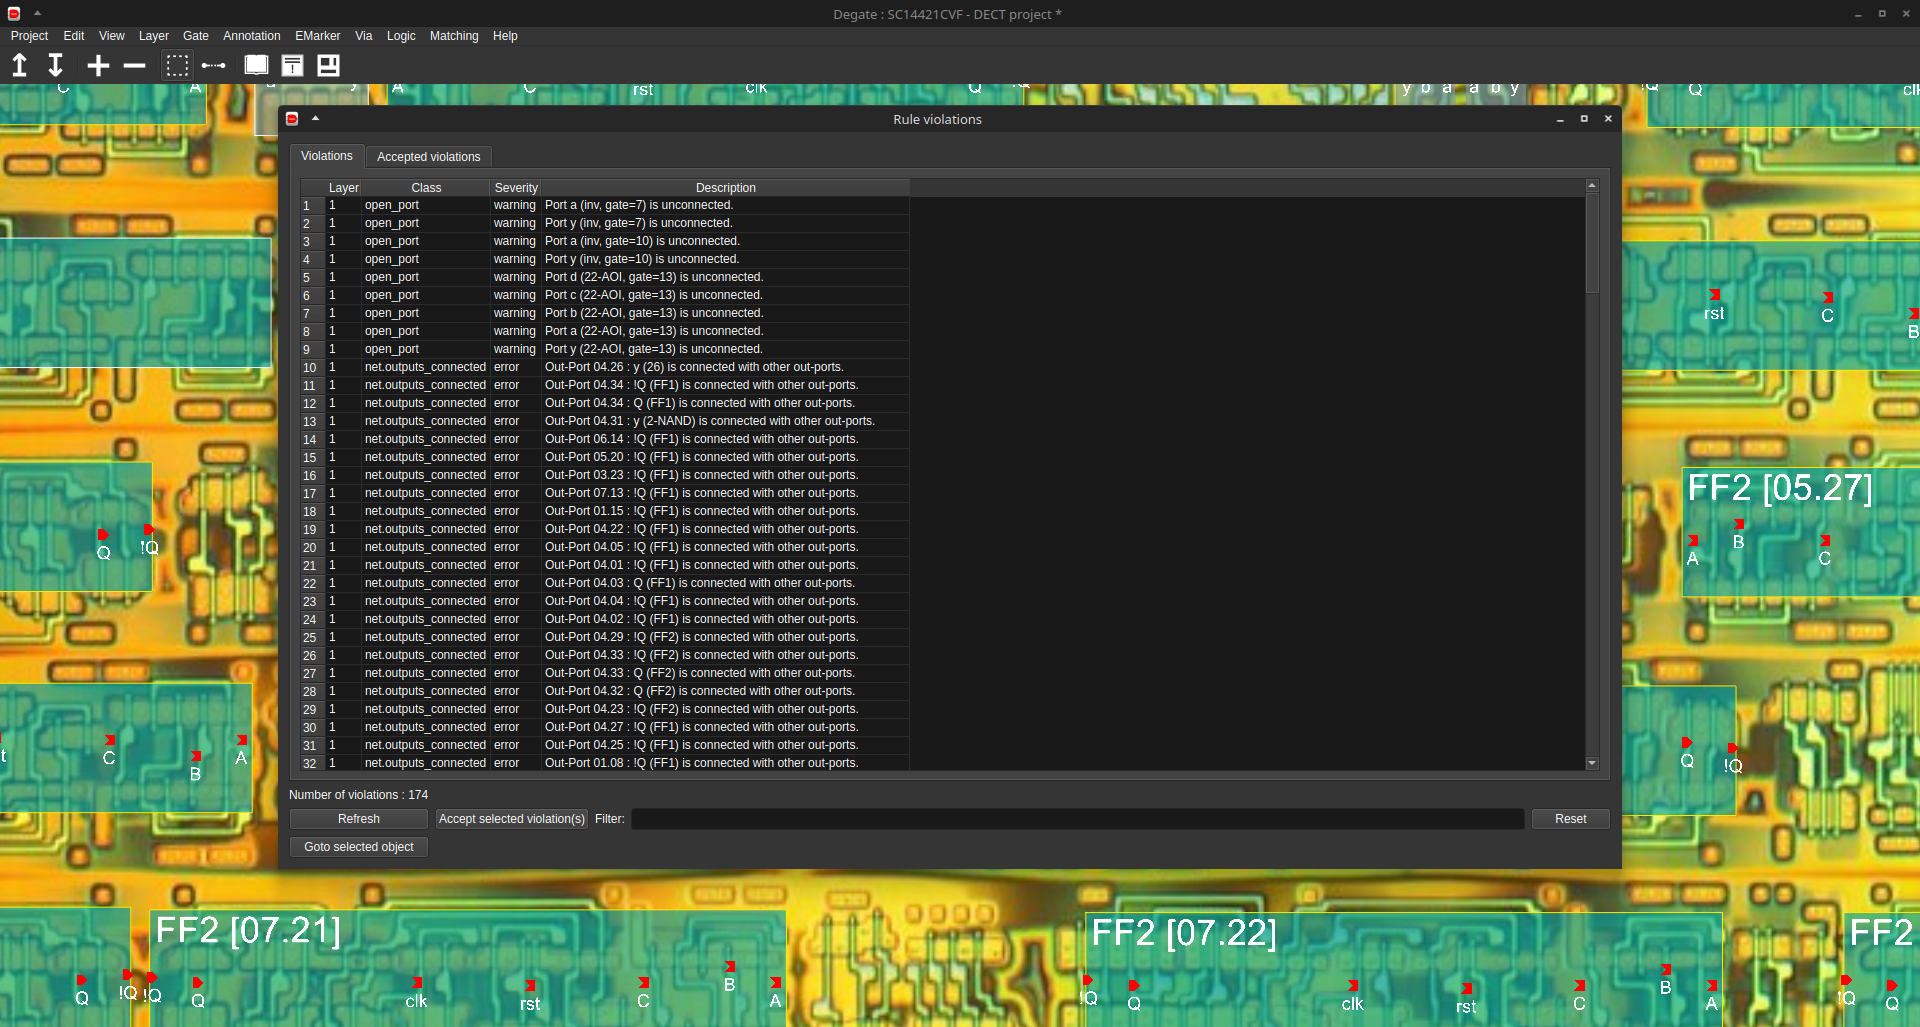
\includegraphics[width=0.8\textwidth]{res/degate_rule.png}
			\end{tabular}
			
			& 
			
			\begin{tabular}{l}
				\hspace{-8mm}
				\parbox{0.225\textwidth}{\footnotesize
					Helpers are available, like rudimentary (but to be improved) rule checking (e.g. for coherency).
				}
			\end{tabular}
		\end{tabular}
	\end{frame}
	%%%%%%%%%%%%%%%%%%%%%%%%%%%%%%%%%%%%%%%%%%%%%%%%%%
	
	%%%%%%%%%%%%%%%%%%%%%%%%%%%%%%%%%%%%%%%%%%%%%%%%%%
	\begin{frame}{Small Demonstration}
			
		\begin{tabular}{cl}  
			
			\begin{tabular}{l}
				\hspace{-8mm}
				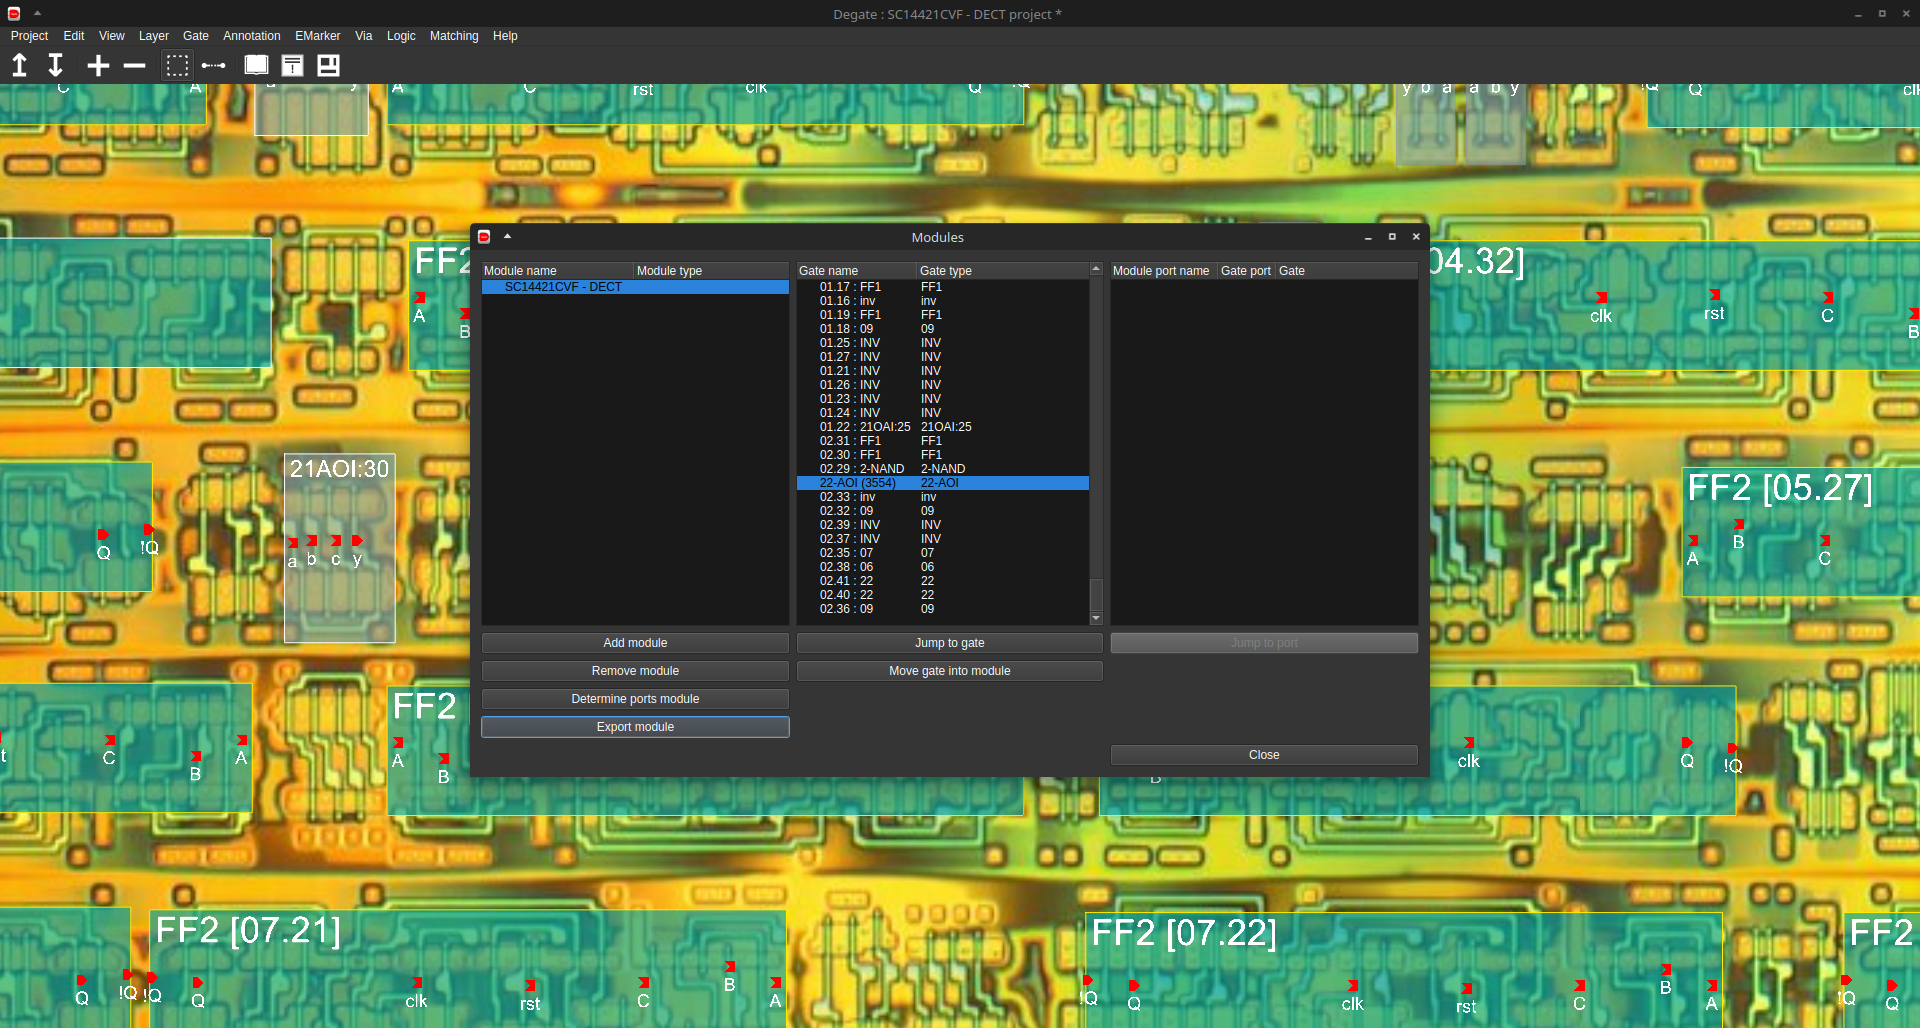
\includegraphics[width=0.8\textwidth]{res/degate_modules.png}
			\end{tabular}
			
			& 
			
			\begin{tabular}{l}
				\hspace{-8mm}
				\parbox{0.225\textwidth}{\footnotesize
					Everything can be organized in "module", exported individually (in Verilog/VHDL), etc... "Divide et impera".
				}
			\end{tabular}
		\end{tabular}
	\end{frame}
	%%%%%%%%%%%%%%%%%%%%%%%%%%%%%%%%%%%%%%%%%%%%%%%%%%
	
	%%%%%%%%%%%%%%%%%%%%%%%%%%%%%%%%%%%%%%%%%%%%%%%%%%
	\begin{frame}{Engineering Challenges}	
		\begin{tabular}{cl}  
			
			\begin{tabular}{l}
				\parbox{0.6\textwidth}{
					\begin{itemize}
						\item Gate template, wires \& vias \textbf{matching}.
						\item Very \textbf{huge images} handling.
						\item \textbf{Error} recovery/acceptance/identification.
						\item Multiple possible \textbf{image format} (e.g. .tiff, .png...) \& \textbf{image source} (e.g. SEM, confocal...).
						\item 10+ years \textbf{old software} (mix of old \& new C++).
						\item \textbf{Collaborative} analysis.
						\item Integrated \textbf{gate analyzer}.
						\item Explicit full \textbf{netlist exporter}.
					\end{itemize}
				}
				
			\end{tabular}
			
			& 
			
			\vspace{8mm}
			\begin{tabular}{cc}
				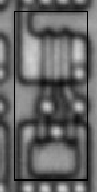
\includegraphics[width=1.55cm]{res/nand_mifare_transistor.png} &
				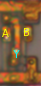
\includegraphics[width=1.45cm]{res/nand_legic_transistor.png} \\
				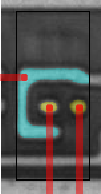
\includegraphics[width=1.48cm]{res/nand_mifare_logic.png} &
				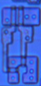
\includegraphics[width=1.45cm]{res/nand_legic_logic.png} \\
				\tiny MIFARE NAND\cite{KarstenNohl2009} &
				\tiny LEGIC NAND\cite{KarstenNohl2009} \\
			\end{tabular}
		\end{tabular}
	\end{frame}
	%%%%%%%%%%%%%%%%%%%%%%%%%%%%%%%%%%%%%%%%%%%%%%%%%%
	
	
	%%%%%%%%%%%%%%%%%%%%%%%%%%%%%%%%%%%%%%%%%%%%%%%%%%
	\begin{frame}{Research Challenges}
		
		\begin{itemize}
			\item \textbf{3D capture}, imply rethinking Degate (New 3D mode? New software? Really accessible?), and \textbf{new algorithms} (e.g. for matching, tracing and gate identification).
			\item \textbf{Machine learning}/better algorithms for:
				\begin{itemize} 
					\item Auto-\textbf{vectorization} ;
					\item Gate auto \textbf{identification} (from vectorized analysis) ;
					\item Gate auto \textbf{wiring} ;
					\item Auto vias \& wires \textbf{identification}.
				\end{itemize}
			\item Take advantage of certain capture methods such as \textbf{SEM} which makes \textbf{automation easier}.
			\item Making the \textbf{field more accessible} (more automation, new abstractions for analysis, communication...).
			\item Use Degate for \textbf{advanced analysis} and \textbf{published results}.
		\end{itemize}

	\end{frame}
	%%%%%%%%%%%%%%%%%%%%%%%%%%%%%%%%%%%%%%%%%%%%%%%%%%
	
%%%%%%%%%%%%%%%%%%%%%%%%%%%%%%%%%%%%%%%%%%%%%%%%%%%%%%%%%%%%%%%%%%%%%%%%%%%%%%%%

%%%%%%%%%%%%%%%%%%%%%%%%%%%%%%%%%%%%%%%%%%%%%%%%%%%%%%%%%%%%%%%%%%%%%%%%%%%%%%%%
%%%%%%%%%%%%%%%%%%%%%%%%%%%%%%%%%%%%%%%%%%%%%%%%%%%%%%%%%%%%%%%%%%%%%%%%%%%%%%%%
%%%%%%%%%%%%%%%%%%%%%%%%%%%%%%%%%%%%%%%%%%%%%%%%%%%%%%%%%%%%%%%%%%%%%%%%%%%%%%%%

\section{MIFARE Classic Chip Reverse Engineering Case}

%%%%%%%%%%%%%%%%%%%%%%%%%%%%%%%%%%%%%%%%%%%%%%%%%%
\begin{frame}{MIFARE Classic Chip \cite{KarstenNohl2009}}
	
	\begin{tabular}{cc}  
		
		\begin{tabular}{c}
			\parbox{0.5\textwidth}{\small
				\vspace{-6mm}
				
				\begin{itemize}
					\item \textbf{RFID card} from NXP launched in 1994.
					\item Used the \textbf{Crypto1 cypher} (until MIFARE Classic EV1, that are using \textbf{Hitag2} cipher).
					\item \textbf{Proprietary encryption} algorithm (stream cipher), security by obscurity.
					\item Cryto1 cipher is only \textbf{implemented in hardware}.
					\item Used (back in 2008) in more than \textbf{3.5 billions cards} (including many building access control systems).
				\end{itemize}
				
				\vspace{3mm}
				
				A \textbf{huge target} with a \textbf{suspicious cypher} and \textbf{security standards}?
			}
		\end{tabular}
		
		& 

		\begin{tabular}{c}
			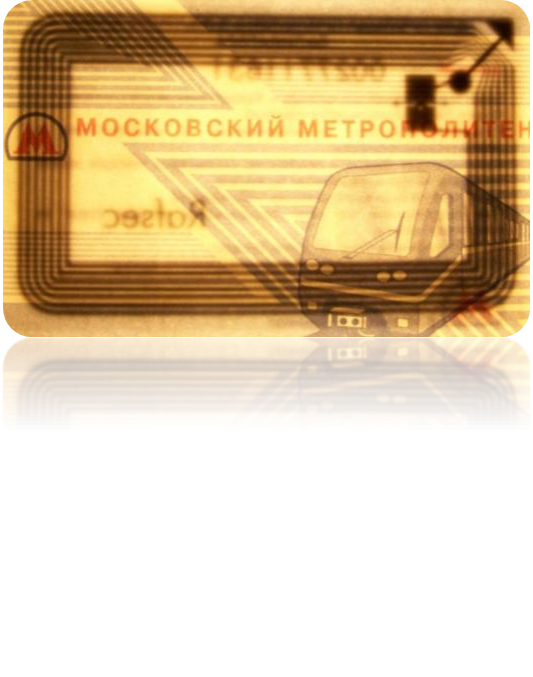
\includegraphics[width=0.4\textwidth]{res/mifare.png}
		\end{tabular}
	\end{tabular}
\end{frame}
%%%%%%%%%%%%%%%%%%%%%%%%%%%%%%%%%%%%%%%%%%%%%%%%%%

%%%%%%%%%%%%%%%%%%%%%%%%%%%%%%%%%%%%%%%%%%%%%%%%%%
\begin{frame}{Degate's origins \cite{NohlEvans2008}}
	
	\begin{tabular}{cc}  
		
		\begin{tabular}{c}
			\hspace{-7mm}
			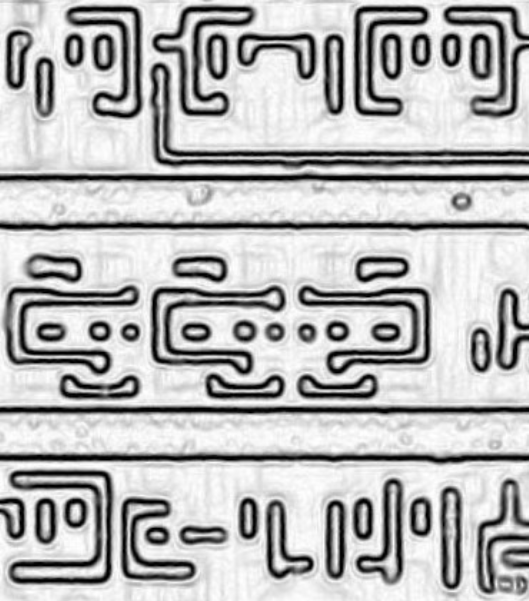
\includegraphics[width=0.4\textwidth]{res/mifare_reverse2.png}
		\end{tabular}
		
		& 
		
		\begin{tabular}{c}
			
			\hspace{-10mm}
			\parbox{0.6\textwidth}{\footnotesize
				\begin{itemize}
					\item K. Nohl \& Starbug \textbf{reverse-engineered the Crypto1 cypher} from MIFARE Classic chip in 2007.
					\item Used \textbf{acetone} to dissolve the RFID cards.
					\item Used \textbf{manual polishing} for delayering.
					\item Image a total of \textbf{6 layers}.
					\item Identify zone of interest, \textbf{searching for 48-bit register} \& group of XOR gates.
					\item Used \textbf{standard optical microscope} (500x) \& hugin tool for stitching.
					\item Identified \textbf{around 70 types of gates}.
					\item Used \textbf{home-made scripts} (which became the base of Degate) for \textbf{template matching} to identify all gates.
					\item \textbf{Manually} reconstructed \textbf{connections} between gates.
					\item Made a \textbf{script} to help detecting \textbf{wires} \& \textbf{vias}.
				\end{itemize}
			}
		\end{tabular}
	\end{tabular}
\end{frame}
%%%%%%%%%%%%%%%%%%%%%%%%%%%%%%%%%%%%%%%%%%%%%%%%%%

%%%%%%%%%%%%%%%%%%%%%%%%%%%%%%%%%%%%%%%%%%%%%%%%%%
\begin{frame}{Consequences \cite{NohlEvans2008}}
	\begin{tabular}{cc}  
		\hspace{-10mm}
		\parbox{0.6\textwidth}{\footnotesize
			\begin{itemize}
				\item Using the reverse-engineering results and protocol analysis, authors found \textbf{multiple weakness} in the cipher:
				\begin{itemize}
					\item The cipher is vulnerable to \textbf{brute force} attack, key is too small.
					\item RNG is predictable, it uses a 16-bit LFSR (linear feedback shift register) \textbf{initialized with constant value} and reset at each power-up.
					\item There is \textbf{only one secret key} for each ID that can result to a specific session key, and all shifts are linear.
				\end{itemize}
				\item Meaning that just by \textbf{sniffing interactions} with the card and the reader, we can compute the key and \textbf{retrieve all the data} of the card.
				\item NXP release a retro-compatible \& "hardened" version of the Cipher (Hitag2), which was also weak, MIFARE Classic were \textbf{"discontinued" in 2015}.
			\end{itemize}
		}
		
		& 
		
		\begin{tabular}{c}
			\begin{tabular}{c}
				\hspace{-7mm}
				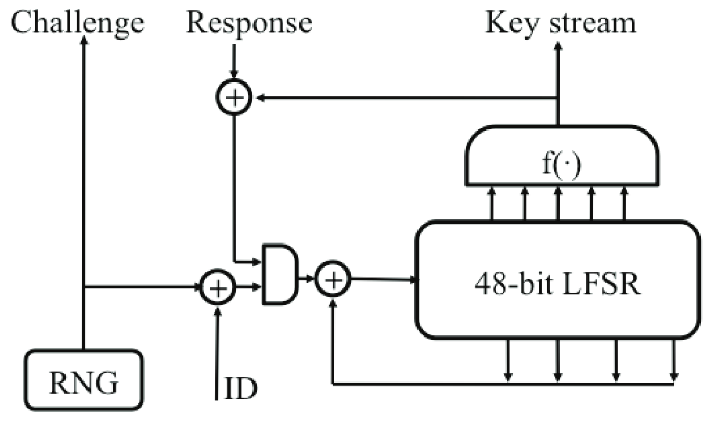
\includegraphics[width=0.4\textwidth]{res/crypto1.png}
			\end{tabular} \\
			\hspace{-10mm}
			\parbox{0.35\textwidth}{\footnotesize
				\begin{itemize}
					\item Authors \textbf{analyzed other RFID devices} after.
					\item \textbf{Degate was created} from this analysis, used for other RFID devices reverse-engineering and open-sourced in 2008.
				\end{itemize}
			}
		\end{tabular}
	\end{tabular}
\end{frame}
%%%%%%%%%%%%%%%%%%%%%%%%%%%%%%%%%%%%%%%%%%%%%%%%%%

%%%%%%%%%%%%%%%%%%%%%%%%%%%%%%%%%%%%%%%%%%%%%%%%%%%%%%%%%%%%%%%%%%%%%%%%%%%%%%%%
%%%%%%%%%%%%%%%%%%%%%%%%%%%%%%%%%%%%%%%%%%%%%%%%%%%%%%%%%%%%%%%%%%%%%%%%%%%%%%%%
%%%%%%%%%%%%%%%%%%%%%%%%%%%%%%%%%%%%%%%%%%%%%%%%%%%%%%%%%%%%%%%%%%%%%%%%%%%%%%%%

\section{Future of Silicon Chip Reverse Engineering}

%%%%%%%%%%%%%%%%%%%%%%%%%%%%%%%%%%%%%%%%%%%%%%%%%%
\begin{frame}{Future of Silicon Chip RE}
	\begin{itemize}
		\item \textbf{Simpler} and \textbf{cheaper} IC capture (decap \& delayer).
		\item Making the \textbf{field more accessible} (communication, more real-life and useful example/reference analysis...).
		\item \textbf{Shared and open} library of \textbf{chips captures} ($\sim$zeptobar \& siliconpr0n + SiliconZoo).
		\item \textbf{Machine learning} to automate even more analysis steps (\textit{gate identification, wire extract, algorithm retrieving \& analysis})?
	\end{itemize}

	\vspace{3mm}

	There is \textbf{2 EU projects} running around \textbf{ICs reverse-engineering}, but no information on tools, process and analysis \underline{\textbf{sharing}}.
	
	\begin{center}
		\begin{tabular}{cccc}  
			
			\hspace{-13mm}
			
			\begin{tabular}{c}
				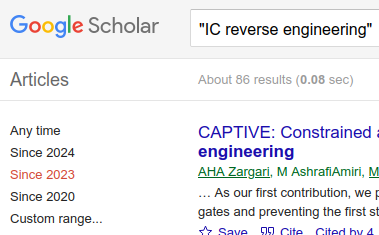
\includegraphics[width=0.27\textwidth]{res/google_scholar.png}
			\end{tabular}
			
			& 
			
			\begin{tabular}{c}
				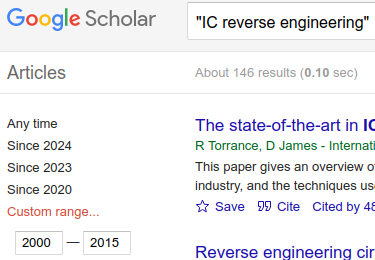
\includegraphics[width=0.25\textwidth]{res/old_google_scholar.png}
			\end{tabular}
			
			& 
			
			\hspace{10mm}
			
			\begin{tabular}{c}
				
\includegraphics[width=0.1\textwidth]{res/ForRES.png}
			\end{tabular}
			
			& 
			
			\begin{tabular}{c}
				
\includegraphics[width=0.1\textwidth]{res/ORSHIN.png}
			\end{tabular}
			
		\end{tabular}
	\end{center}
\end{frame}
%%%%%%%%%%%%%%%%%%%%%%%%%%%%%%%%%%%%%%%%%%%%%%%%%%

%%%%%%%%%%%%%%%%%%%%%%%%%%%%%%%%%%%%%%%%%%%%%%%%%%%%%%%%%%%%%%%%%%%%%%%%%%%%%%%%
%%%%%%%%%%%%%%%%%%%%%%%%%%%%%%%%%%%%%%%%%%%%%%%%%%%%%%%%%%%%%%%%%%%%%%%%%%%%%%%%
%%%%%%%%%%%%%%%%%%%%%%%%%%%%%%%%%%%%%%%%%%%%%%%%%%%%%%%%%%%%%%%%%%%%%%%%%%%%%%%%

\section{Bonus}

%%%%%%%%%%%%%%%%%%%%%%%%%%%%%%%%%%%%%%%%%%%%%%%%%%
\begin{frame}{Which gate is this?}
	% This is a nand, inversed on y axis
	
	\begin{center}
		\begin{tabular}{ccc}
			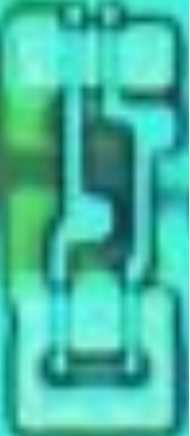
\includegraphics[width=2.6cm]{res/nand2_transistor_a.png} &
			\includegraphics[width=2.6cm]{res/nand2_logic_a.png} &
			\includegraphics[width=2.6cm]{res/nand2_metal_a.png} \\
			\tiny Transistor layer &
			\tiny Logic layer &
			\tiny Metal layer \\
		\end{tabular}
	\end{center}
\end{frame}
%%%%%%%%%%%%%%%%%%%%%%%%%%%%%%%%%%%%%%%%%%%%%%%%%%

%%%%%%%%%%%%%%%%%%%%%%%%%%%%%%%%%%%%%%%%%%%%%%%%%%%%%%%%%%%%%%%%%%%%%%%%%%%%%%%%
%%%%%%%%%%%%%%%%%%%%%%%%%%%%%%%%%%%%%%%%%%%%%%%%%%%%%%%%%%%%%%%%%%%%%%%%%%%%%%%%
%%%%%%%%%%%%%%%%%%%%%%%%%%%%%%%%%%%%%%%%%%%%%%%%%%%%%%%%%%%%%%%%%%%%%%%%%%%%%%%%

\section{References}

%%%%%%%%%%%%%%%%%%%%%%%%%%%%%%%%%%%%%%%%%%%%%%%%%%
\begin{frame}[allowframebreaks]{References}
	\bibliographystyle{plain}
	\bibliography{bibli}
	\nocite{*}
\end{frame}
%%%%%%%%%%%%%%%%%%%%%%%%%%%%%%%%%%%%%%%%%%%%%%%%%%

%%%%%%%%%%%%%%%%%%%%%%%%%%%%%%%%%%%%%%%%%%%%%%%%%%%%%%%%%%%%%%%%%%%%%%%%%%%%%%%%
%%%%%%%%%%%%%%%%%%%%%%%%%%%%%%%%%%%%%%%%%%%%%%%%%%%%%%%%%%%%%%%%%%%%%%%%%%%%%%%%
%%%%%%%%%%%%%%%%%%%%%%%%%%%%%%%%%%%%%%%%%%%%%%%%%%%%%%%%%%%%%%%%%%%%%%%%%%%%%%%%

\end{document}
